\documentclass{zkdl-presentation-template}

\title[Projective Space and Pairing]{\textbf{Projective Coordinates and Pairing}}
\author{Distributed Lab}
\date{August 8, 2024}
\homepage{zkdl-camp.github.io}
\github{ZKDL-Camp}

\begin{document}
    \frame {
        \tikz [remember picture,overlay]
        \node at
            ([yshift=1.5cm,xshift=-1.5cm]current page.south east) 
            %or: (current page.center)
            {
\includegraphics[width=60pt]{images/logo.png}};
        \titlepage
    }
 
	\begin{frame}{Plan}
        \tableofcontents
    \end{frame}

	\section{Affine Coordinates Issue: Recap}

    \subsection{Recap}
    \begin{frame}{Elliptic Curve Definition}
        \begin{definition}
            Suppose that $\mathbb{K}$ is a field. An \textbf{elliptic curve} $E$ over $\mathbb{K}$ is defined as a set of points $(x,y) \in \mathbb{K}^2$:
            \vspace{-5pt}
            \begin{equation*}
                y^2 = x^3+ax+b,
            \end{equation*}
            \vspace{-20pt}

            called a \textbf{Short Weierstrass equation}, where $a,b \in \mathbb{K}$ and $4a^3+27b^2 \neq 0$. $E/\mathbb{K}$ denotes the elliptic curve over field $\mathbb{K}$.
        \end{definition}

        \begin{block}{Definition}
            Point $P \in E(\overline{\mathbb{F}}_p)$, represented by coordinates $(x_P,y_P)$ is called the \textbf{affine representation} of $P$ and denoted as $P \in \mathbb{A}^2(\overline{\mathbb{F}}_p)$.
        \end{block}

        \begin{definition}
            $E(\mathbb{K}) = E/\mathbb{K} \cup \{\mathcal{O}\}$. $(E(\mathbb{K}), \oplus)$ forms a group, where $\oplus$ is the \textbf{point addition} operation.
        \end{definition}
    \end{frame}

    \begin{frame}{Addition and Doubling Illustratins}
        \begin{figure}
            \centering
            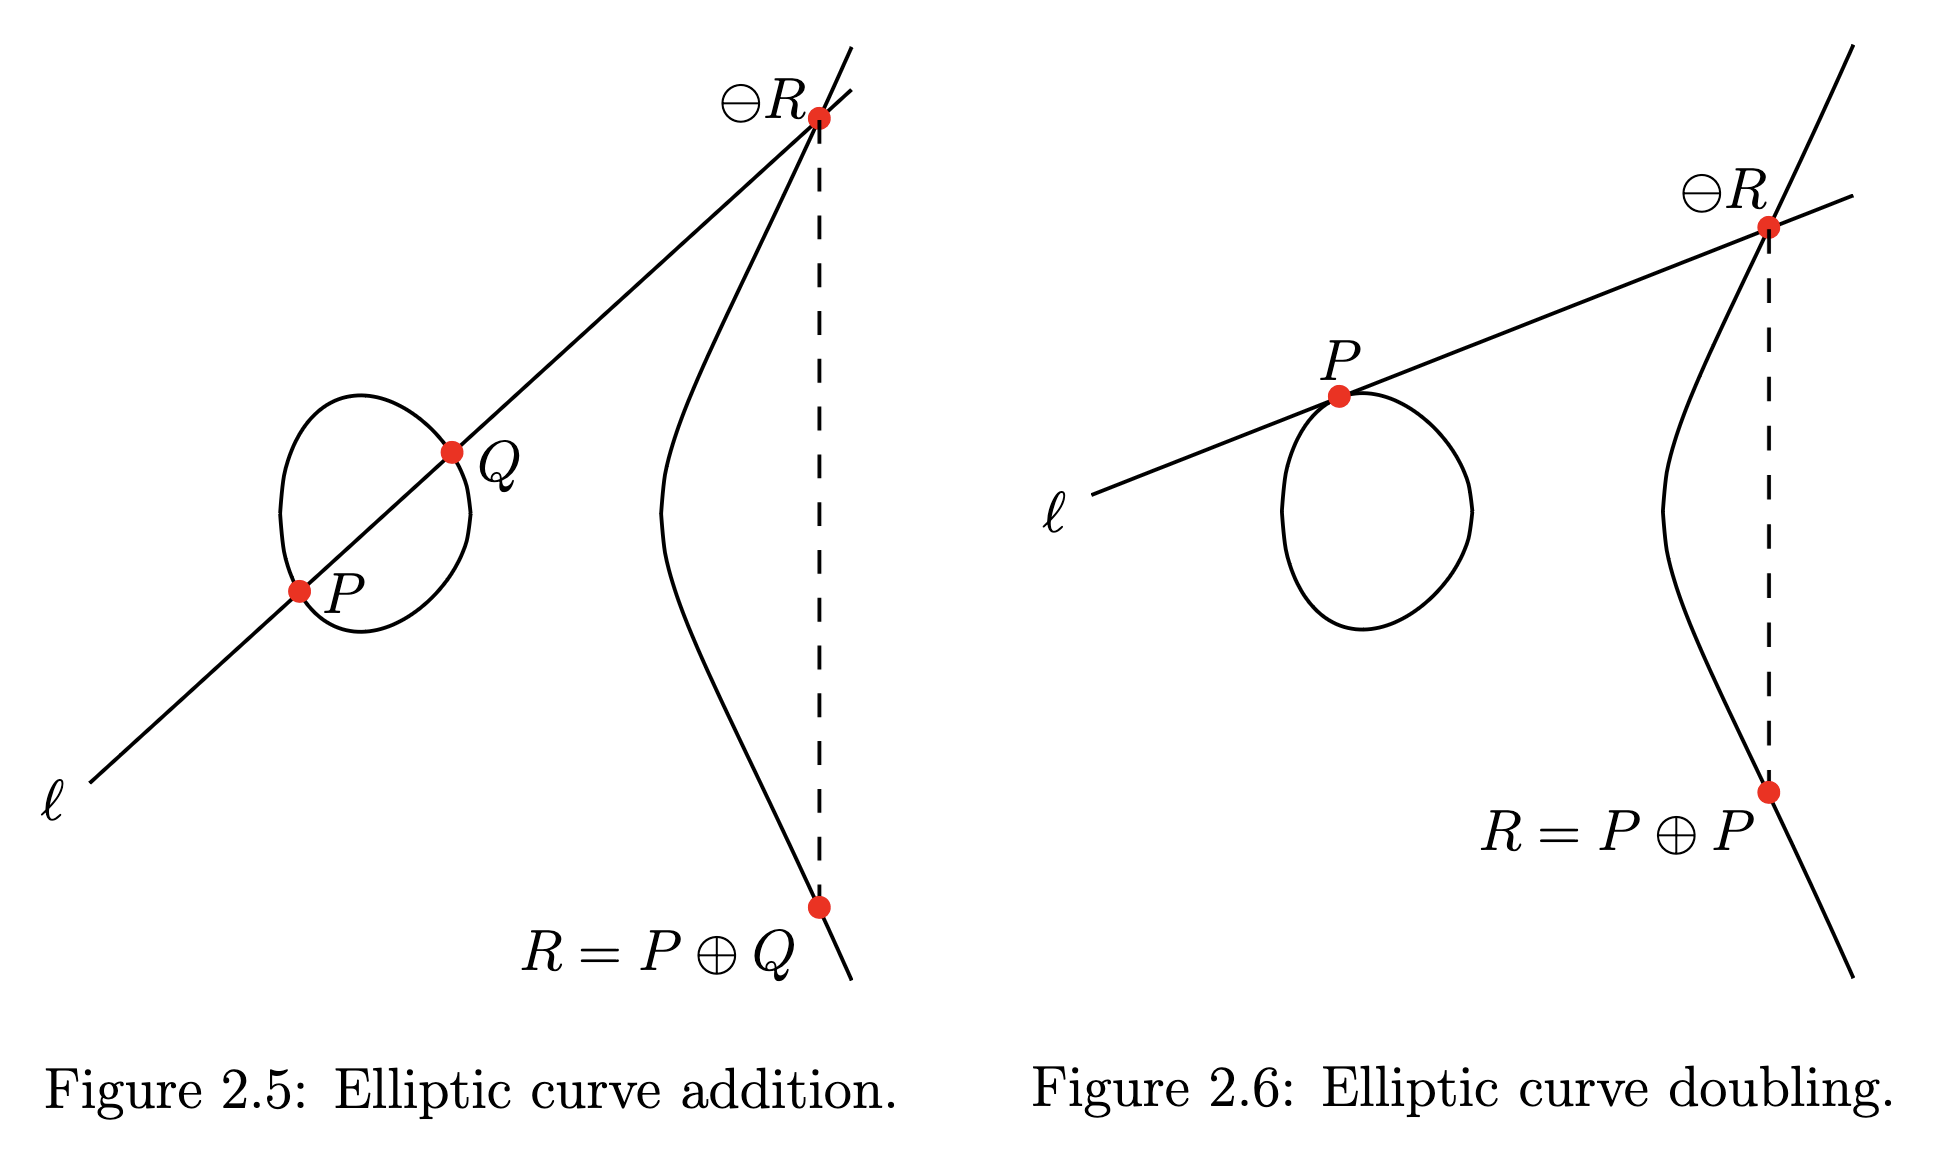
\includegraphics[width=0.9\textwidth]{images/lecture_4/addition.png}
            \caption{Illustration of chord-and-tangent points addition.}
        \end{figure}
    \end{frame}

    \begin{frame}{Affine Point Addition}
        So, how do we add $(x_R,y_R) = (x_P,y_P) \oplus (x_Q,y_Q)$ where $(x_P,y_P)$ and $(x_Q,y_Q)$ are affine representation of points $P,Q \in E(\overline{\mathbb{F}}_p)$?
        
        \begin{block}{Algorithm 1: Classical adding $P$ and $Q$ for $x_P \neq x_Q$}
        \begin{enumerate}
           \item Calculate the slope $
                \lambda \gets (y_P-y_Q)/(x_P-x_Q)$. 
           \item Set 
           \begin{equation*}
           x_R \gets \lambda^2 - x_P - x_Q, \;\; y_R \gets \lambda(x_P - x_R) - y_P.
           \end{equation*}
        \end{enumerate}
        \end{block}

        Easy, right? What can go wrong?
    \end{frame}

    \subsection{Addition Complexity}
    \begin{frame}{Why this is bad?}
        \begin{columns}
            % -- Description --
            \begin{column}{0.5\textwidth}
            Let 
            \begin{itemize}
                \item $\textcolor{oc-indigo-8}{\boldsymbol{M}}$ --- cost of multiplication;
                \item $\textcolor{oc-green-8}{\boldsymbol{S}}$ --- cost of squaring;
                \item $\textcolor{oc-red-7}{\boldsymbol{I}}$ --- cost of inverse.
            \end{itemize}

            (all in some extension $\mathbb{F}_{p^m}$)
        \end{column}
        \begin{column}{0.5\textwidth}
            \textbf{Algorithm 1:} Calculating $P \oplus Q$
            \begin{gather*}
                \lambda \gets (y_P-y_Q)\textcolor{oc-indigo-8}{\times}(x_P-x_Q)^{\textcolor{oc-red-7}{-1}} \\
                x_R \gets \lambda^{\textcolor{oc-green-8}{2}} - x_P - x_Q \\
                y_R \gets \lambda \textcolor{oc-indigo-8}{\times} (x_P - x_R) - y_P
            \end{gather*}
        \end{column}
        \end{columns}
        \vspace{10px}
        Then, calculating the aforementioned formula costs:
        \begin{equation*}
            2\textcolor{oc-indigo-8}{\boldsymbol{M}} + \textcolor{oc-green-8}{\boldsymbol{S}} + \textcolor{oc-red-7}{\boldsymbol{I}}
        \end{equation*}

        Well, just 4 operations... Easy right?

        \begin{alertblock}{Main Problem!}
            Typically, $\boldsymbol{I} \approx 80\boldsymbol{M}$. So, the effective cost is roughly \textbf{80 operations}. Too bad. We need to fix it!
        \end{alertblock}
    \end{frame}

    \section{Relations}
    \subsection{Definition}
    \begin{frame}{Relation}
        Our solution would be \textbf{projective coordinates}, but we need a couple of ingredients first.

        \begin{definition}
            Let $\mathcal{X},\mathcal{Y}$ be some sets. Then, $\mathcal{R}$ is a \textbf{relation} if 
            \begin{equation*}
                \mathcal{R} \subset \mathcal{X} \times \mathcal{Y} = \{(x,y): x \in \mathcal{X}, y \in \mathcal{Y}\}
            \end{equation*}
        \end{definition}
        
        \begin{example}
            Let $\mathcal{X} = \{\text{Oleksandr}, \text{Phat}, \text{Anton}\}$, $\mathcal{Y} = \{\text{Backend}, \text{Frontend}, \text{Research}\}$. Define the following relation of ``person $x$ works in field $y$'':
            \begin{equation*}
                \mathcal{R} = \{(\text{Oleksandr}, \text{Research}), (\text{Phat}, \text{Frontend}), (\text{Anton}, \text{Backend})\}
            \end{equation*}
            Obviously, $\mathcal{R} \subset \mathcal{X} \times \mathcal{Y}$, so $\mathcal{R}$ is a relation.
        \end{example}
    \end{frame}

    \subsection{Equivalence Relation}
    \begin{frame}{Equivalence Relation}
        \begin{definition}
            Let $\mathcal{X}$ be a set. A relation $\sim$ on $\mathcal{X}$ is called an \textbf{equivalence relation} if it satisfies the following properties:
            \begin{enumerate}
                \item \textbf{Reflexivity:} $x \sim x$ for all $x \in \mathcal{X}$.
                \item \textbf{Symmetry:} If $x \sim y$, then $y \sim x$ for all $x,y \in \mathcal{X}$.
                \item \textbf{Transitivity:} If $x \sim y$ and $y \sim z$, then $x \sim z$ for all $x,y,z \in \mathcal{X}$.
            \end{enumerate}
        \end{definition}
        
        \begin{example}
            Let $\mathcal{X}$ be the set of all people. Define a relation $\sim$ on $\mathcal{X}$ by $x \sim y$ if $x,y \in \mathcal{X}$ have the same birthday. 
            Then $\sim$ is an equivalence relation on $\mathcal{X}$.
            \begin{enumerate}
                \item \textbf{Reflexivity:} $x \sim x$ since $x$ has the same birthday as $x$.
                \item \textbf{Symmetry:} If $x \sim y$, then $y \sim x$ (obvious).
                \item \textbf{Transitivity:} If $x \sim y$ and $y \sim z$, then $x \sim z$.
            \end{enumerate}
        \end{example}
    \end{frame}

    \begin{frame}{Equivalence Relation: More Examples}
        \begin{example}
            Suppose $\mathcal{X} = \mathbb{Z}$ and $n$ is some fixed integer. Let $a \sim b$ mean that $a \equiv b \pmod{n}$. It is easy to verify that $\sim$ is an equivalence relation:
            \begin{enumerate}
                \item \textbf{Reflexivity:} $a \equiv a \pmod{n}$, so $a \sim a$.
                \item \textbf{Symmetry:} If $a \equiv b \pmod{n}$, then $b \equiv a \pmod{n}$, so $b \sim a$.
                \item \textbf{Transitivity:} If $a \equiv b \pmod{n}$ and $b \equiv c \pmod{n}$, then $a \equiv c \pmod{n}$, so $(a \sim b) \wedge (b \sim c) \implies a \sim c$.
            \end{enumerate}
        \end{example}

        \begin{example}
            Isomorphism $\cong$ is an equivalence relation on the set of all groups.
        \end{example}

        \begin{alertblock}{Question}
            For $\mathbb{R}$ define $a \sim b \; \text{iff} \; a \geq b$. Is it an equivalence relation?
        \end{alertblock}
    \end{frame}

    \begin{frame}{Equivalence Classes}
        Notice that for the set of integers $\mathbb{Z}$ and relation $\sim$ defined by $a \sim b$ iff $a \equiv b \pmod{n}$, we can group all integers into equivalence classes. For example, for $n=2$:
        \begin{equation*}
            \mathbb{Z} = \{a \in \mathbb{Z}: \text{$a$ is even}\} \cup \{a \in \mathbb{Z}: \text{$a$ is odd}\}
        \end{equation*}

        Can we generalize this observation for general relations?

        \begin{definition}
            Let $\mathcal{X}$ be a set and $\sim$ be an equivalence relation on $\mathcal{X}$. For any $x \in \mathcal{X}$, the \textbf{equivalence class} of $x$ is the set
            \begin{equation*}
                [x] = \{y \in \mathcal{X}: x \sim y\}
            \end{equation*}
             The \textbf{set of all equivalence classes} is denoted by $\mathcal{X}/\text{$\sim$}$ (or, if the relation $\mathcal{R}$ is given explicitly, then $\mathcal{X}/\mathcal{R}$), which is read as ``$\mathcal{X}$ modulo relation $\sim$''.
        \end{definition}
    \end{frame}

    \begin{frame}{Equivalence Classes Properties}
        \begin{example}
            Let $\mathcal{X} = \mathbb{Z}$ and $n$ be some fixed integer. Define $\sim$ on $\mathcal{X}$ by $x \sim y$ if $x \equiv y \pmod{n}$. Then the equivalence class of $x$ is the set
            \begin{equation*}
                [x] = \{y \in \mathbb{Z}: x \equiv y \pmod{n}\}
            \end{equation*}
            For example, $[0] = \{\ldots,-2n,-n,0,n,2n,\ldots\}$ while $[1] = \{\ldots,-2n+1,-n+1,1,n+1,2n+1,\ldots\}$.
        \end{example}
        
        \begin{lemma}
            Let $\mathcal{X}$ be a set and $\sim$ be an equivalence relation on $\mathcal{X}$. Then,
            \begin{enumerate}
                \item For each $x \in \mathcal{X}, x \in [x]$ (quite obvious, follows from reflexivity).
                \item For each $x,y \in \mathcal{X}$, $x \sim y$ if and only if $[x] = [y]$.
                \item For each $x,y \in \mathcal{X}$, either $[x]=[y]$ or $[x] \cap [y] = \emptyset$.
            \end{enumerate}
        \end{lemma}
    \end{frame}

    \begin{frame}{Equivalence Classes Partition Example}
        \begin{example}
            Let $n \in \mathbb{N}$ and, again, $\mathcal{X} = \mathbb{Z}$ with a ``modulo $n$'' equivalence relation $\mathcal{R}_n$. Define the equivalence class of $x$ by $[x]_n = \{y \in \mathbb{Z}: x \equiv y \pmod{n}\}$. Then, 
            \begin{equation*}
                \mathbb{Z}/\mathcal{R}_n = \{[0]_n, [1]_n, [2]_n, \dots, [n-2]_n, [n-1]_n\}
            \end{equation*}
        \end{example}
    \end{frame}

    \section{Elliptic Curve in Projective Coordinates}
    \subsection{Projective Space Definition}

    \begin{frame}{Definition}
        \begin{definition}
            \textbf{Projective coordinate}, denoted as $\mathbb{P}^2(\mathbb{K})$ (or sometimes simply $\mathbb{K}\mathbb{P}^2$) is a set of triplets of elements $(X:Y:Z)$ from $\mathbb{A}^3(\overline{\mathbb{K}}) \setminus \{0\}$ modulo the equivalence relation:
            \begin{gather*}
                (X_1:Y_1:Z_1) \sim (X_2:Y_2:Z_2) \;\; \text{iff} \\\exists \lambda \in \overline{\mathbb{K}}^{\times}: (X_1:Y_1:Z_1) = (\lambda X_2: \lambda Y_2: \lambda Z_2)
            \end{gather*}
        \end{definition}
        
        \begin{example}
            Consider the projective space $\mathbb{P}^2(\mathbb{R})$. Then, two points $(x_1,y_1,z_1),(x_2,y_2,z_2) \in \mathbb{R}^3$ are equivalent if there exists $\lambda \in \mathbb{R}\setminus \{0\}$ such that $(x_1,y_1,z_1) = (\lambda x_2, \lambda y_2, \lambda z_2)$. For example, $(1,2,3) \sim (2,4,6)$ since $(1,2,3) = (0.5 \times 2,0.5 \times 4,0.5 \times 6)$, so $\lambda = 0.5$.
        \end{example}
    \end{frame}

    \begin{frame}{Illustration}
        \begin{example}
            Now, how to geometrically interpret $\mathbb{P}^2(\mathbb{R})$? Consider the Figure below.
        
            \begin{center}
                \begin{tabular}{cc}
                    \centering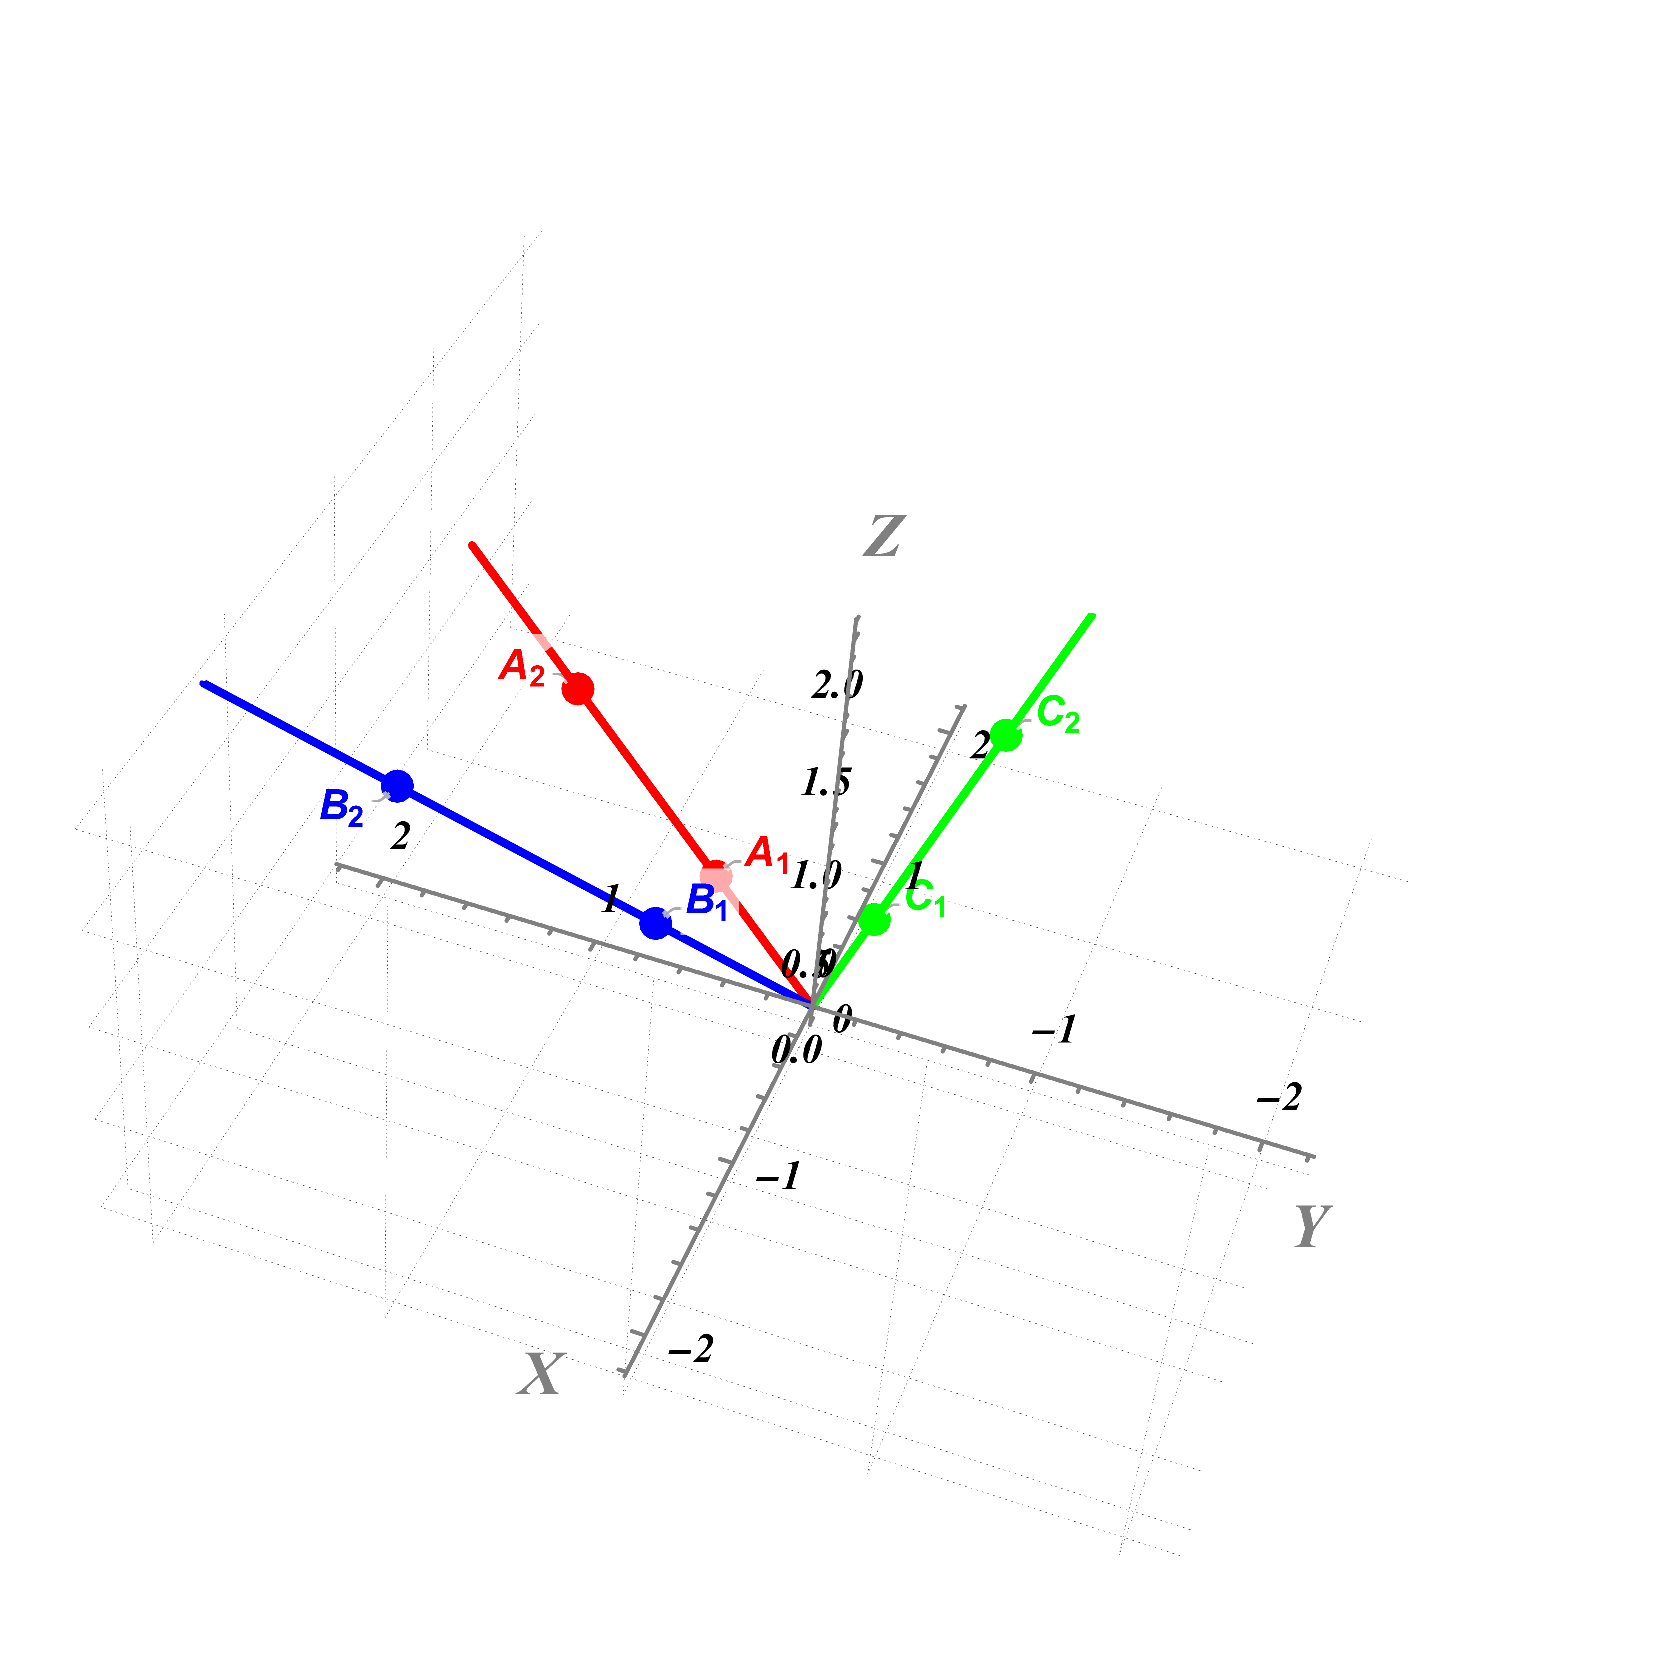
\includegraphics[trim={100 100 100 200}, width=0.45\linewidth, clip]{images/lecture_4/line_1_view_1.pdf} &
                    \centering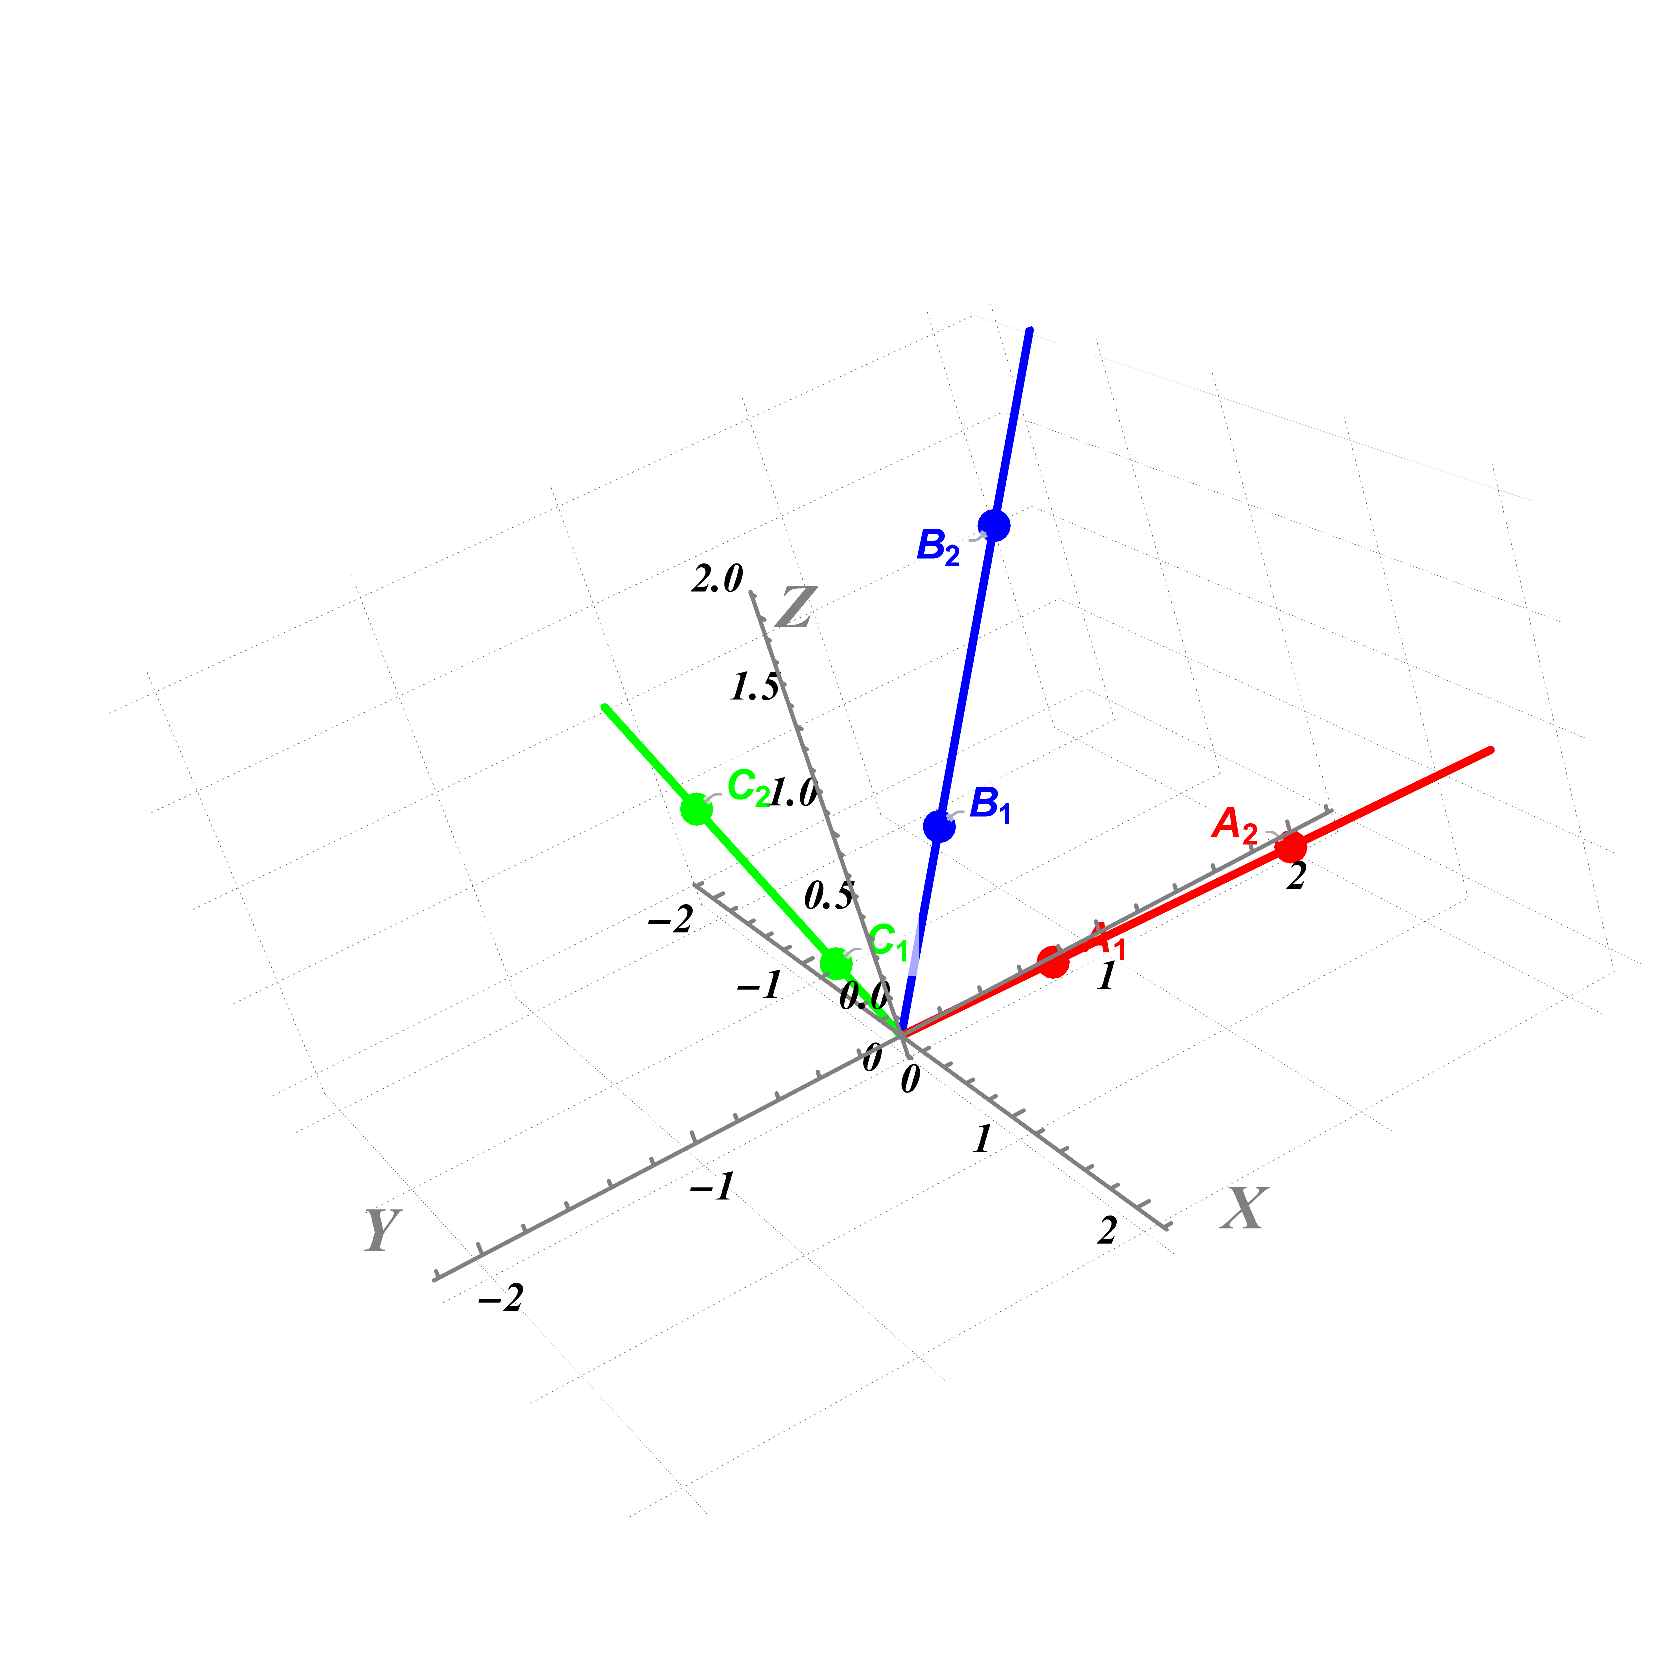
\includegraphics[trim={100 100 100 200}, width=0.45\linewidth, clip]{images/lecture_4/line_1_view_2.pdf}
                \end{tabular}
            \end{center}

            Equivalent points lie on the same line through the origin $(0,0,0)$.
        \end{example}
    \end{frame}

    \begin{frame}{Questions}
        \begin{alertblock}{Question \#1}
            Are points $(1,2,3)$ and $(3,6,9)$ equivalent in $\mathbb{P}^2(\mathbb{R})$?
        \end{alertblock}

        \begin{alertblock}{Question \#2}
            Are points $(1,2,3)$ and $(2,3,1)$ equivalent in $\mathbb{P}^2(\mathbb{R})$?
        \end{alertblock}

        \begin{alertblock}{Question \#3}
            Are points $(2,4,6)$ and $(3,6,9)$ equivalent in $\mathbb{P}^2(\mathbb{R})$?
        \end{alertblock}
    \end{frame}

    \begin{frame}{Going back to Affine Space}
        \begin{block}{Observation \#1}
            Define the map $\phi: \mathbb{P}^2(\mathbb{K}) \to \mathbb{A}^2(\mathbb{K})$ as $\phi(X:Y:Z) = (X/Z,Y/Z)$ for $(X:Y:Z) \in \mathbb{P}^2(\mathbb{K})$. This map will map all equivalent points (lying on the same line) to the same point in $\mathbb{A}^2(\mathbb{K})$.
        \end{block}

       \begin{block}{Observation \#2}
            Define the map $\psi: \mathbb{A}^2(\mathbb{K}) \to \mathbb{P}^2(\mathbb{K})$ as $\psi(x,y) = (x:y:1)$. This map will map all points in $\mathbb{A}^2(\mathbb{K})$ to the corresponding equivalence class in $\mathbb{P}^2(\mathbb{K})$.
        \end{block}

        \begin{alertblock}{Question}
            Given point $(2:4:2) \in \mathbb{P}^2(\mathbb{R})$, what is the corresponding point in $\mathbb{A}^2(\mathbb{R})$?
        \end{alertblock}
    \end{frame}

    \begin{frame}{Going back to Affine Space: Illustration}
        \begin{example}
            Again, consider three lines from the previous example. Now, we additionally draw a plane $\pi: z=1$ in our 3-dimensional space (see Illustration below).
        
            \begin{center}
                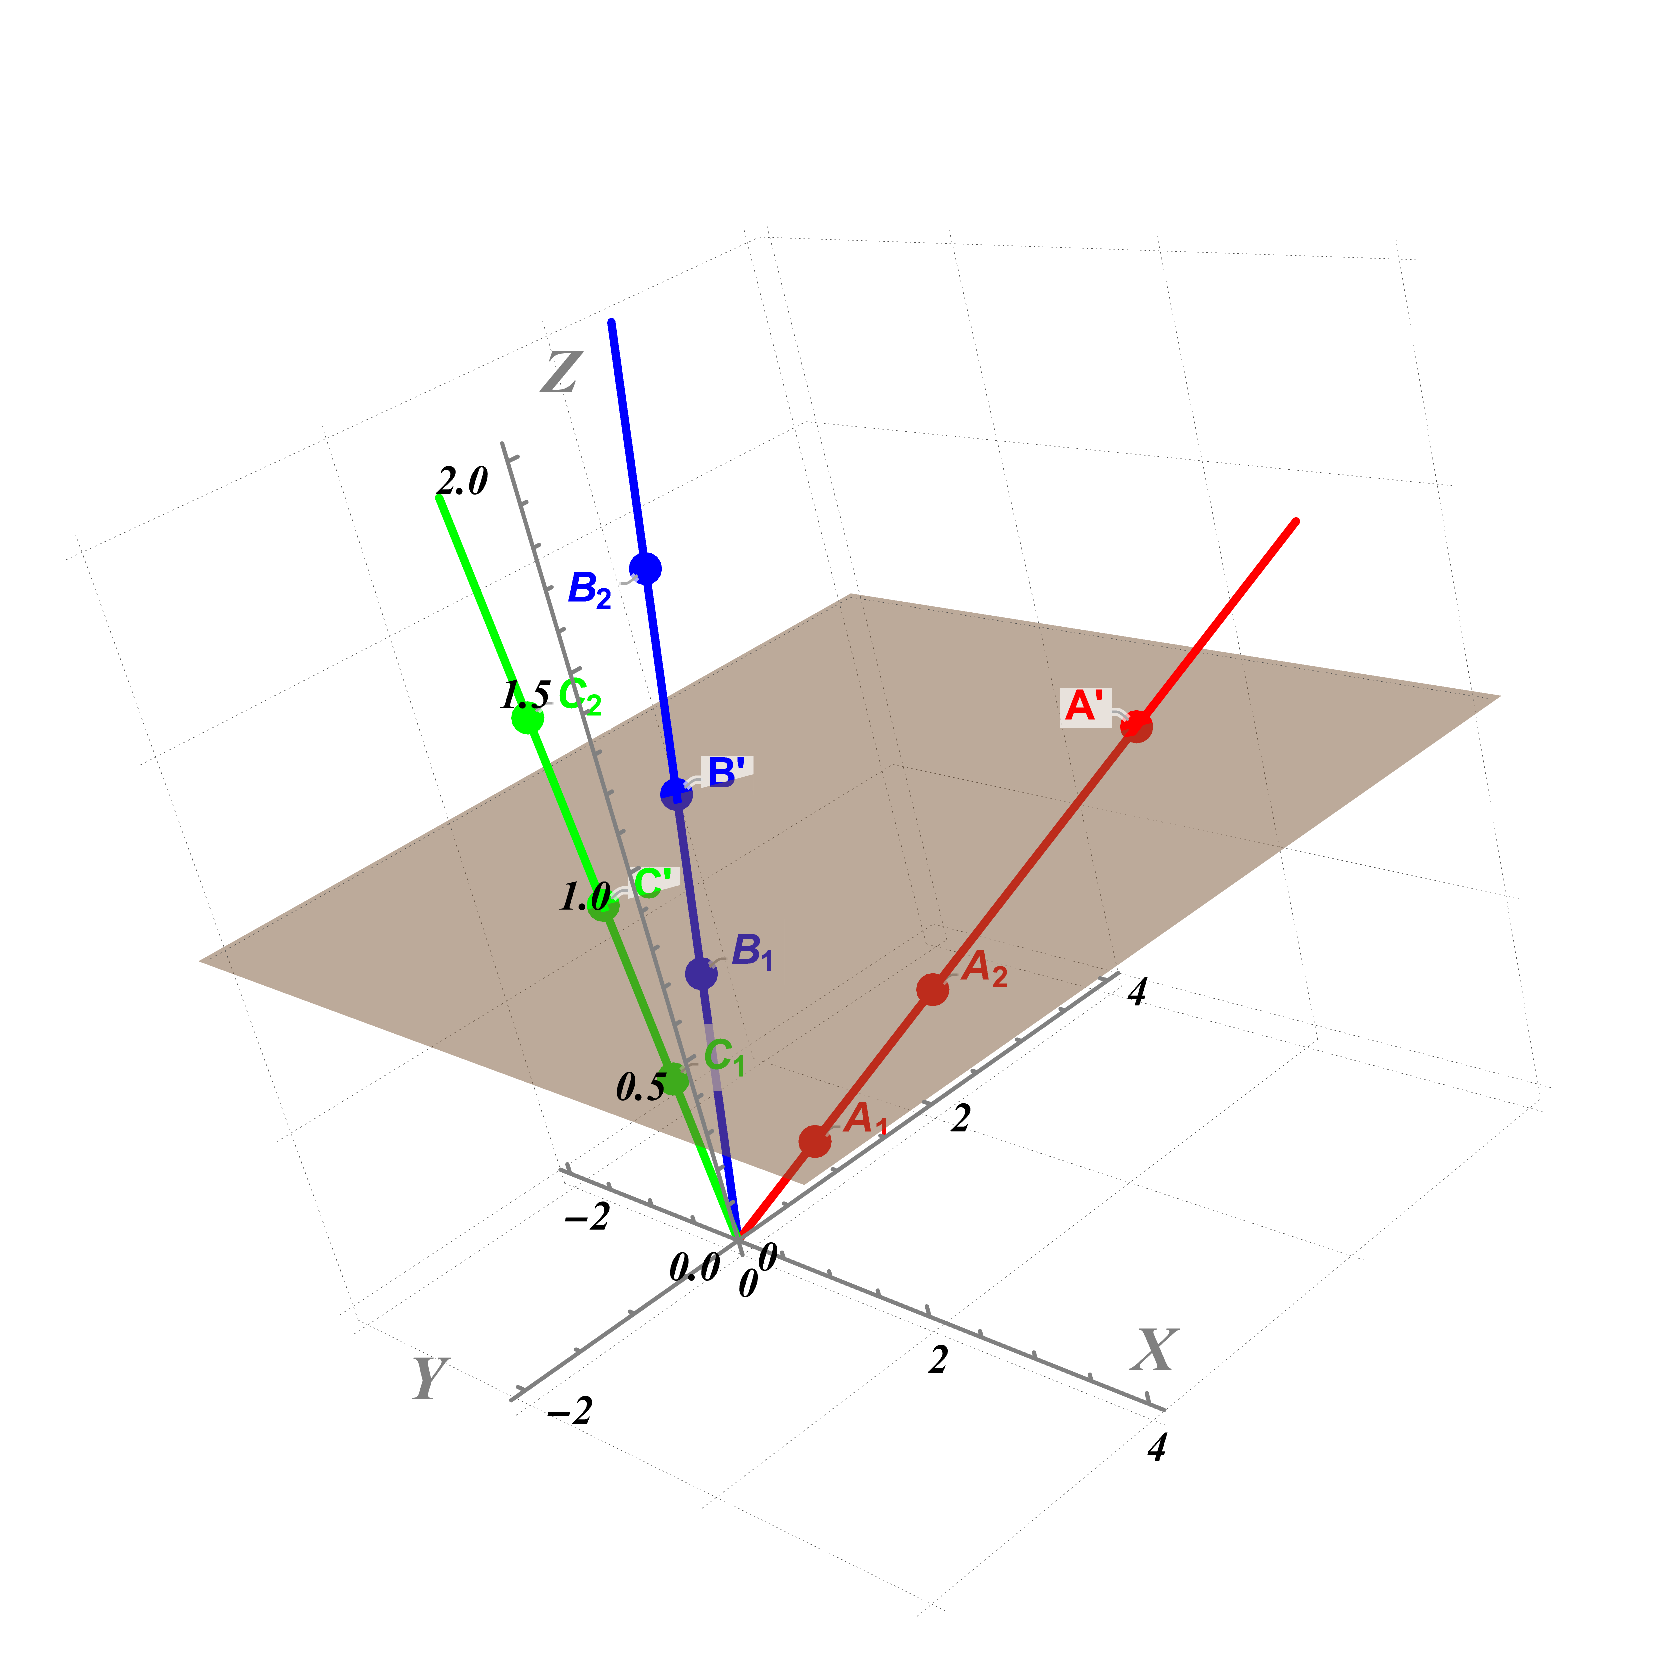
\includegraphics[trim={100 100 100 200}, width=0.45\linewidth, clip]{images/lecture_4/line_2.pdf}
                
                \scriptsize{\textbf{Illustration:} Geometric interpretation of converting projective form to the affine form.}
            \end{center}
        \end{example}
    \end{frame}

    \subsection{Elliptic Curve Equation in Projective Space}
    \begin{frame}{Equation over Projective Space}
        \begin{block}{Observation}
            If $(X:Y:Z)$ lies on the curve, then so does $(X/Z,Y/Z)$.  Thus, since $y^2=x^3+ax+b$ we have:
            \begin{equation*}
                \left(\frac{Y}{Z}\right)^2 = \left(\frac{X}{Z}\right)^3 + a\left(\frac{X}{Z}\right) + b
            \end{equation*}
        \end{block}

        \begin{definition}
            The \textbf{homogeneous projective form} of the elliptic curve is given by the following equation:
            \vspace{-5pt}
            \begin{equation*}
                E_{\mathbb{P}}: Y^2Z = X^3 + aXZ^2 + bZ^3,
            \end{equation*}
            \vspace{-20pt}
            
            where the point at infinity is encoded as $\mathcal{O} = (0:1:0)$.
        \end{definition}

        \begin{block}{Remark}
            Why $\mathcal{O} = (0:1:0)$? Note that all $(0:\lambda:0)$ lie on $E_{\mathbb{P}}$.
        \end{block}
    \end{frame}

    \begin{frame}{Visualization over Projective Space}
        \begin{example}
            Consider the BN254 curve $y^2 = x^3 + 3$ over reals $\mathbb{R}$. Its projective form is given by the equation $Y^2Z = X^3 + 3Z^3$, giving a surface below.
            \begin{center}
                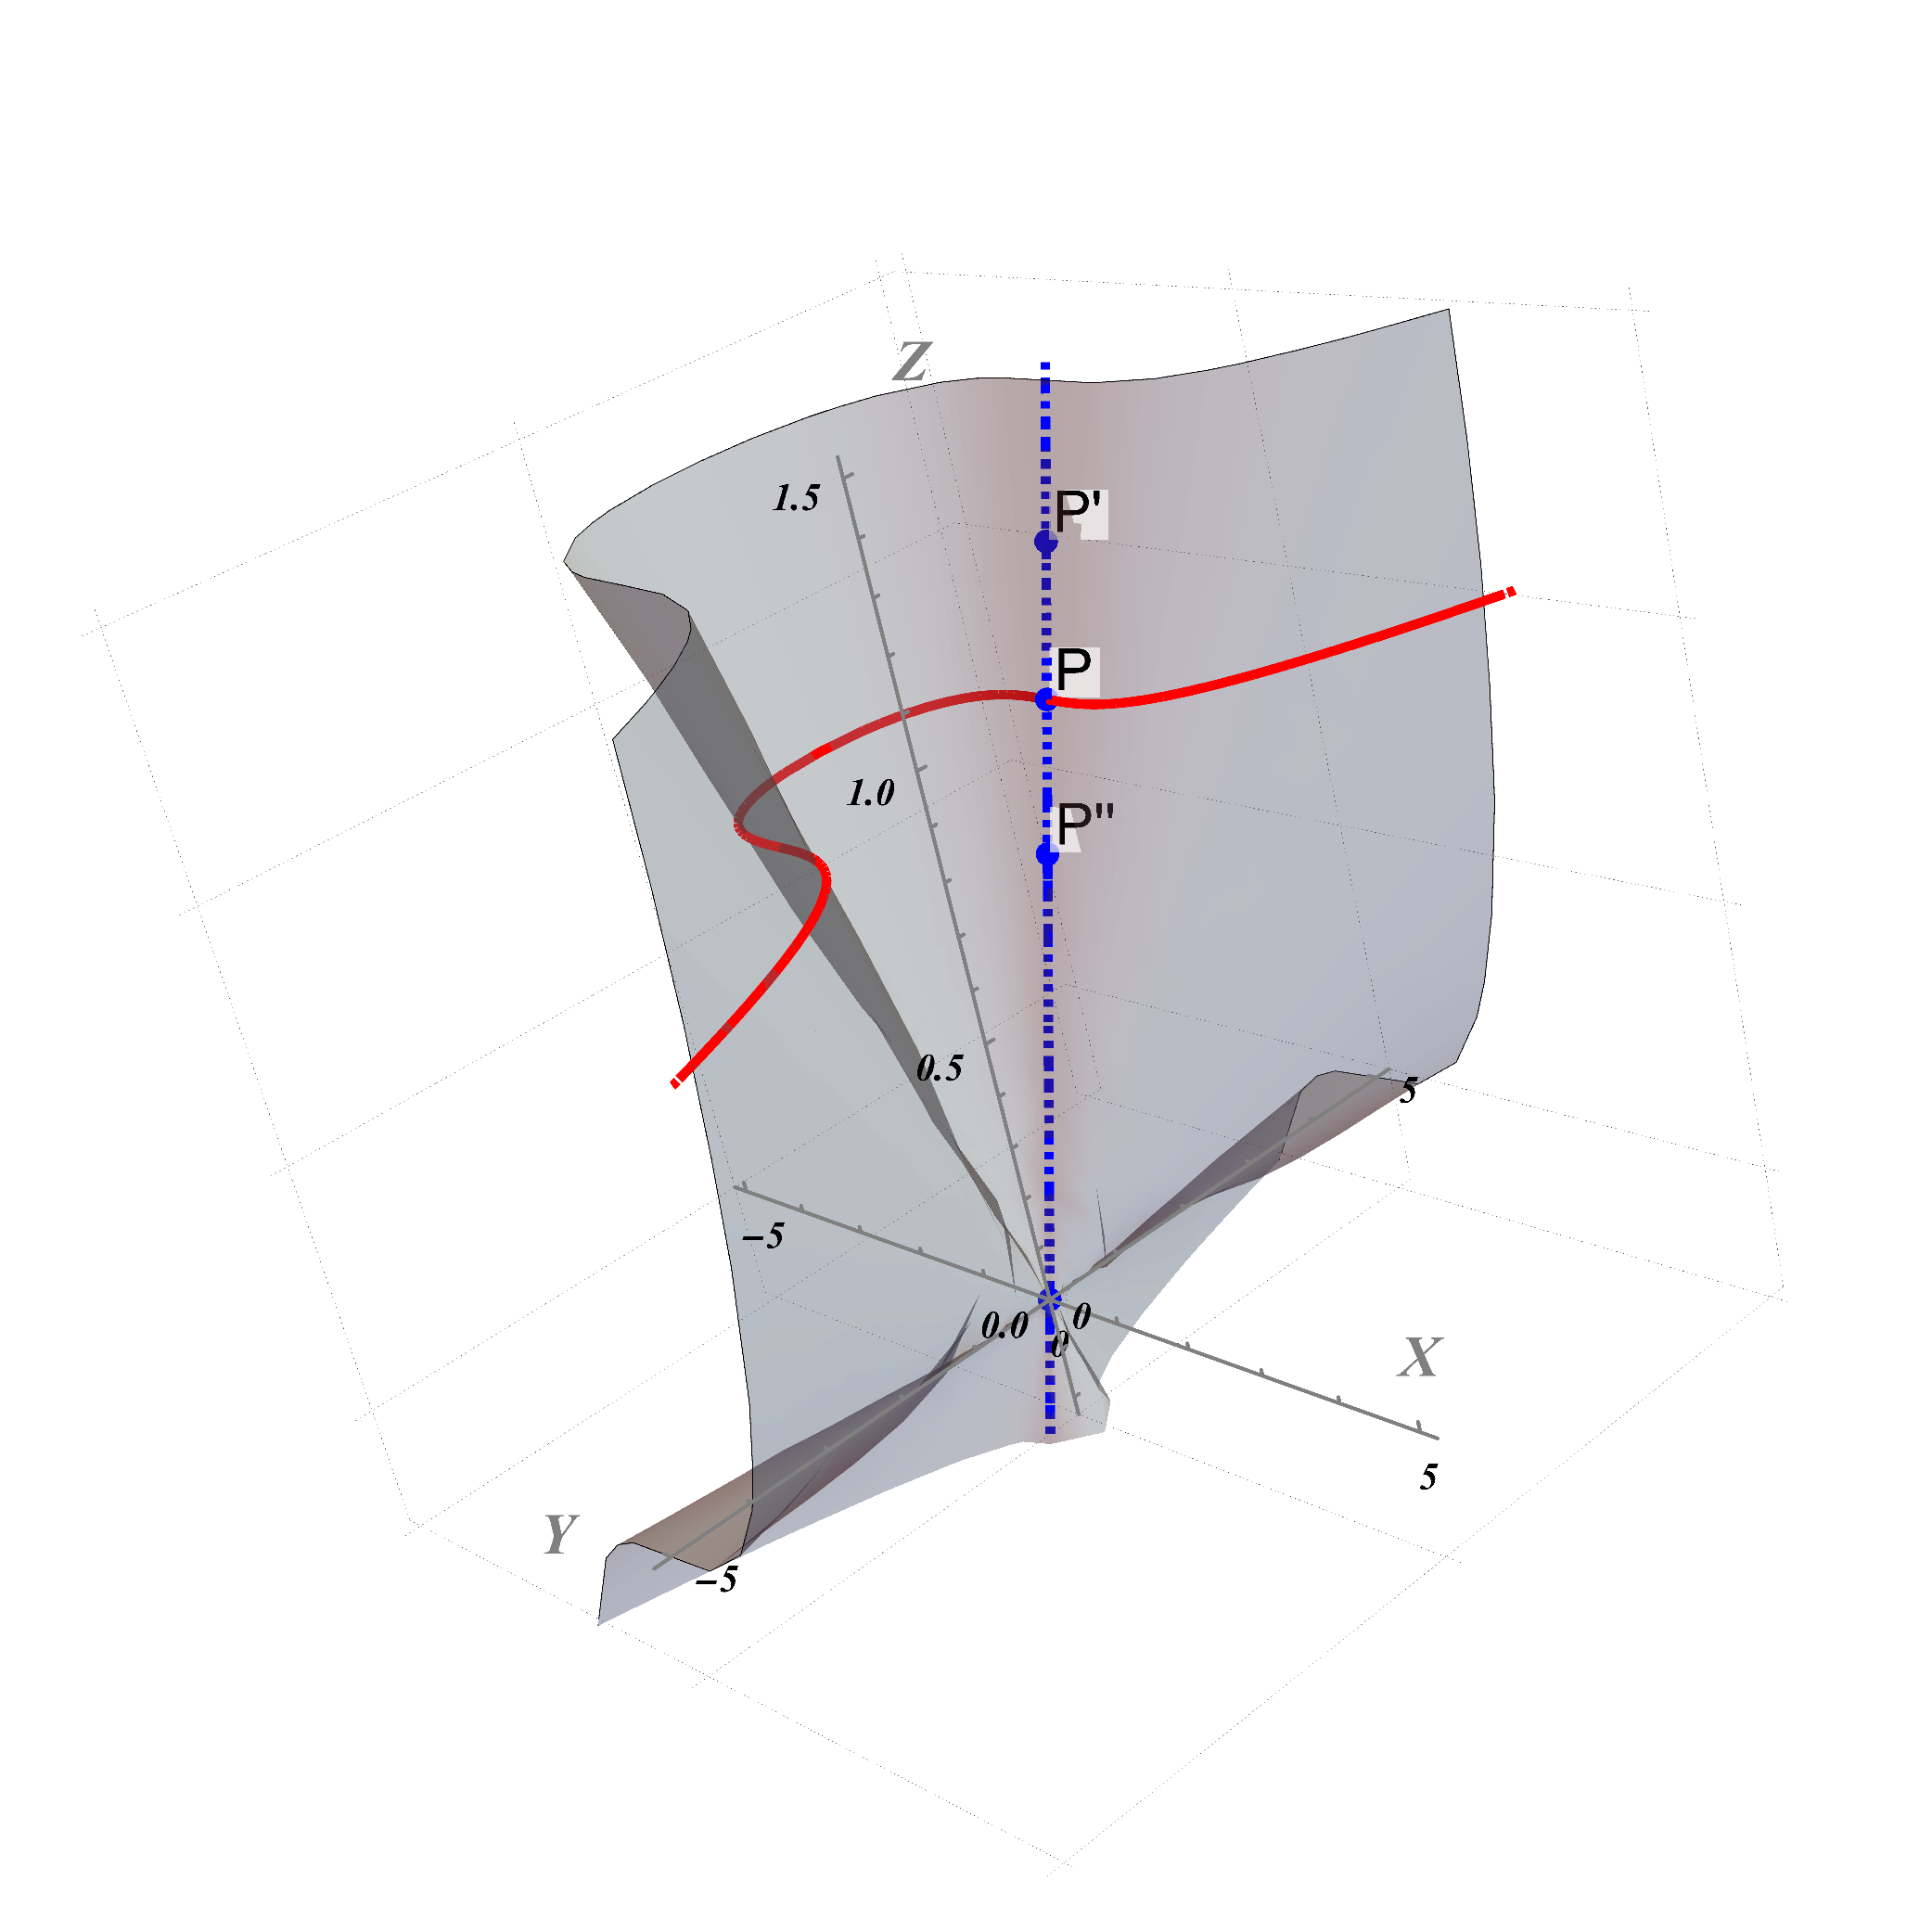
\includegraphics[trim={275 100 225 100}, width=0.3\linewidth, clip]{images/lecture_4/projective_ec.pdf}        
            \end{center}
        \end{example}
    \end{frame}

    \subsection{Projective Addition}

    \begin{frame}{Advantage of Projective Form.}
        \begin{alertblock}{Rhetorical Question}
            Why having three coordinates instead of two is better?
        \end{alertblock}

        Consider the \textbf{addition} operation:
        
        \begin{equation*}
            \begin{aligned}
                X_R = (X_PZ_Q - X_QZ_P)(Z_PZ_Q(Y_PZ_Q-Y_QZ_P)^2\\ - (X_PZ_Q-X_QZ_P)^2(X_PZ_Q+X_QZ_P)); \\
                Y_R = Z_PZ_Q(X_QY_P - X_PY_Q)(X_PZ_Q-X_QZ_P)^2 \\- (Y_PZ_Q-Y_QZ_P)((Y_PZ_Q-Y_QZ_P)^2Z_PZ_Q\\-(X_PZ_Q+X_QZ_P)(X_PZ_Q-X_QZ_P)^2); \\
                Z_R = Z_PZ_Q(X_PZ_Q - X_QZ_P)^3.
            \end{aligned}
        \end{equation*}

         Although looks much more complicated, it takes only \textbf{14M} compared to \textbf{80M}.
    \end{frame}

    \begin{frame}{Illustration of adding two points}	
        \begin{figure}
            \centering
            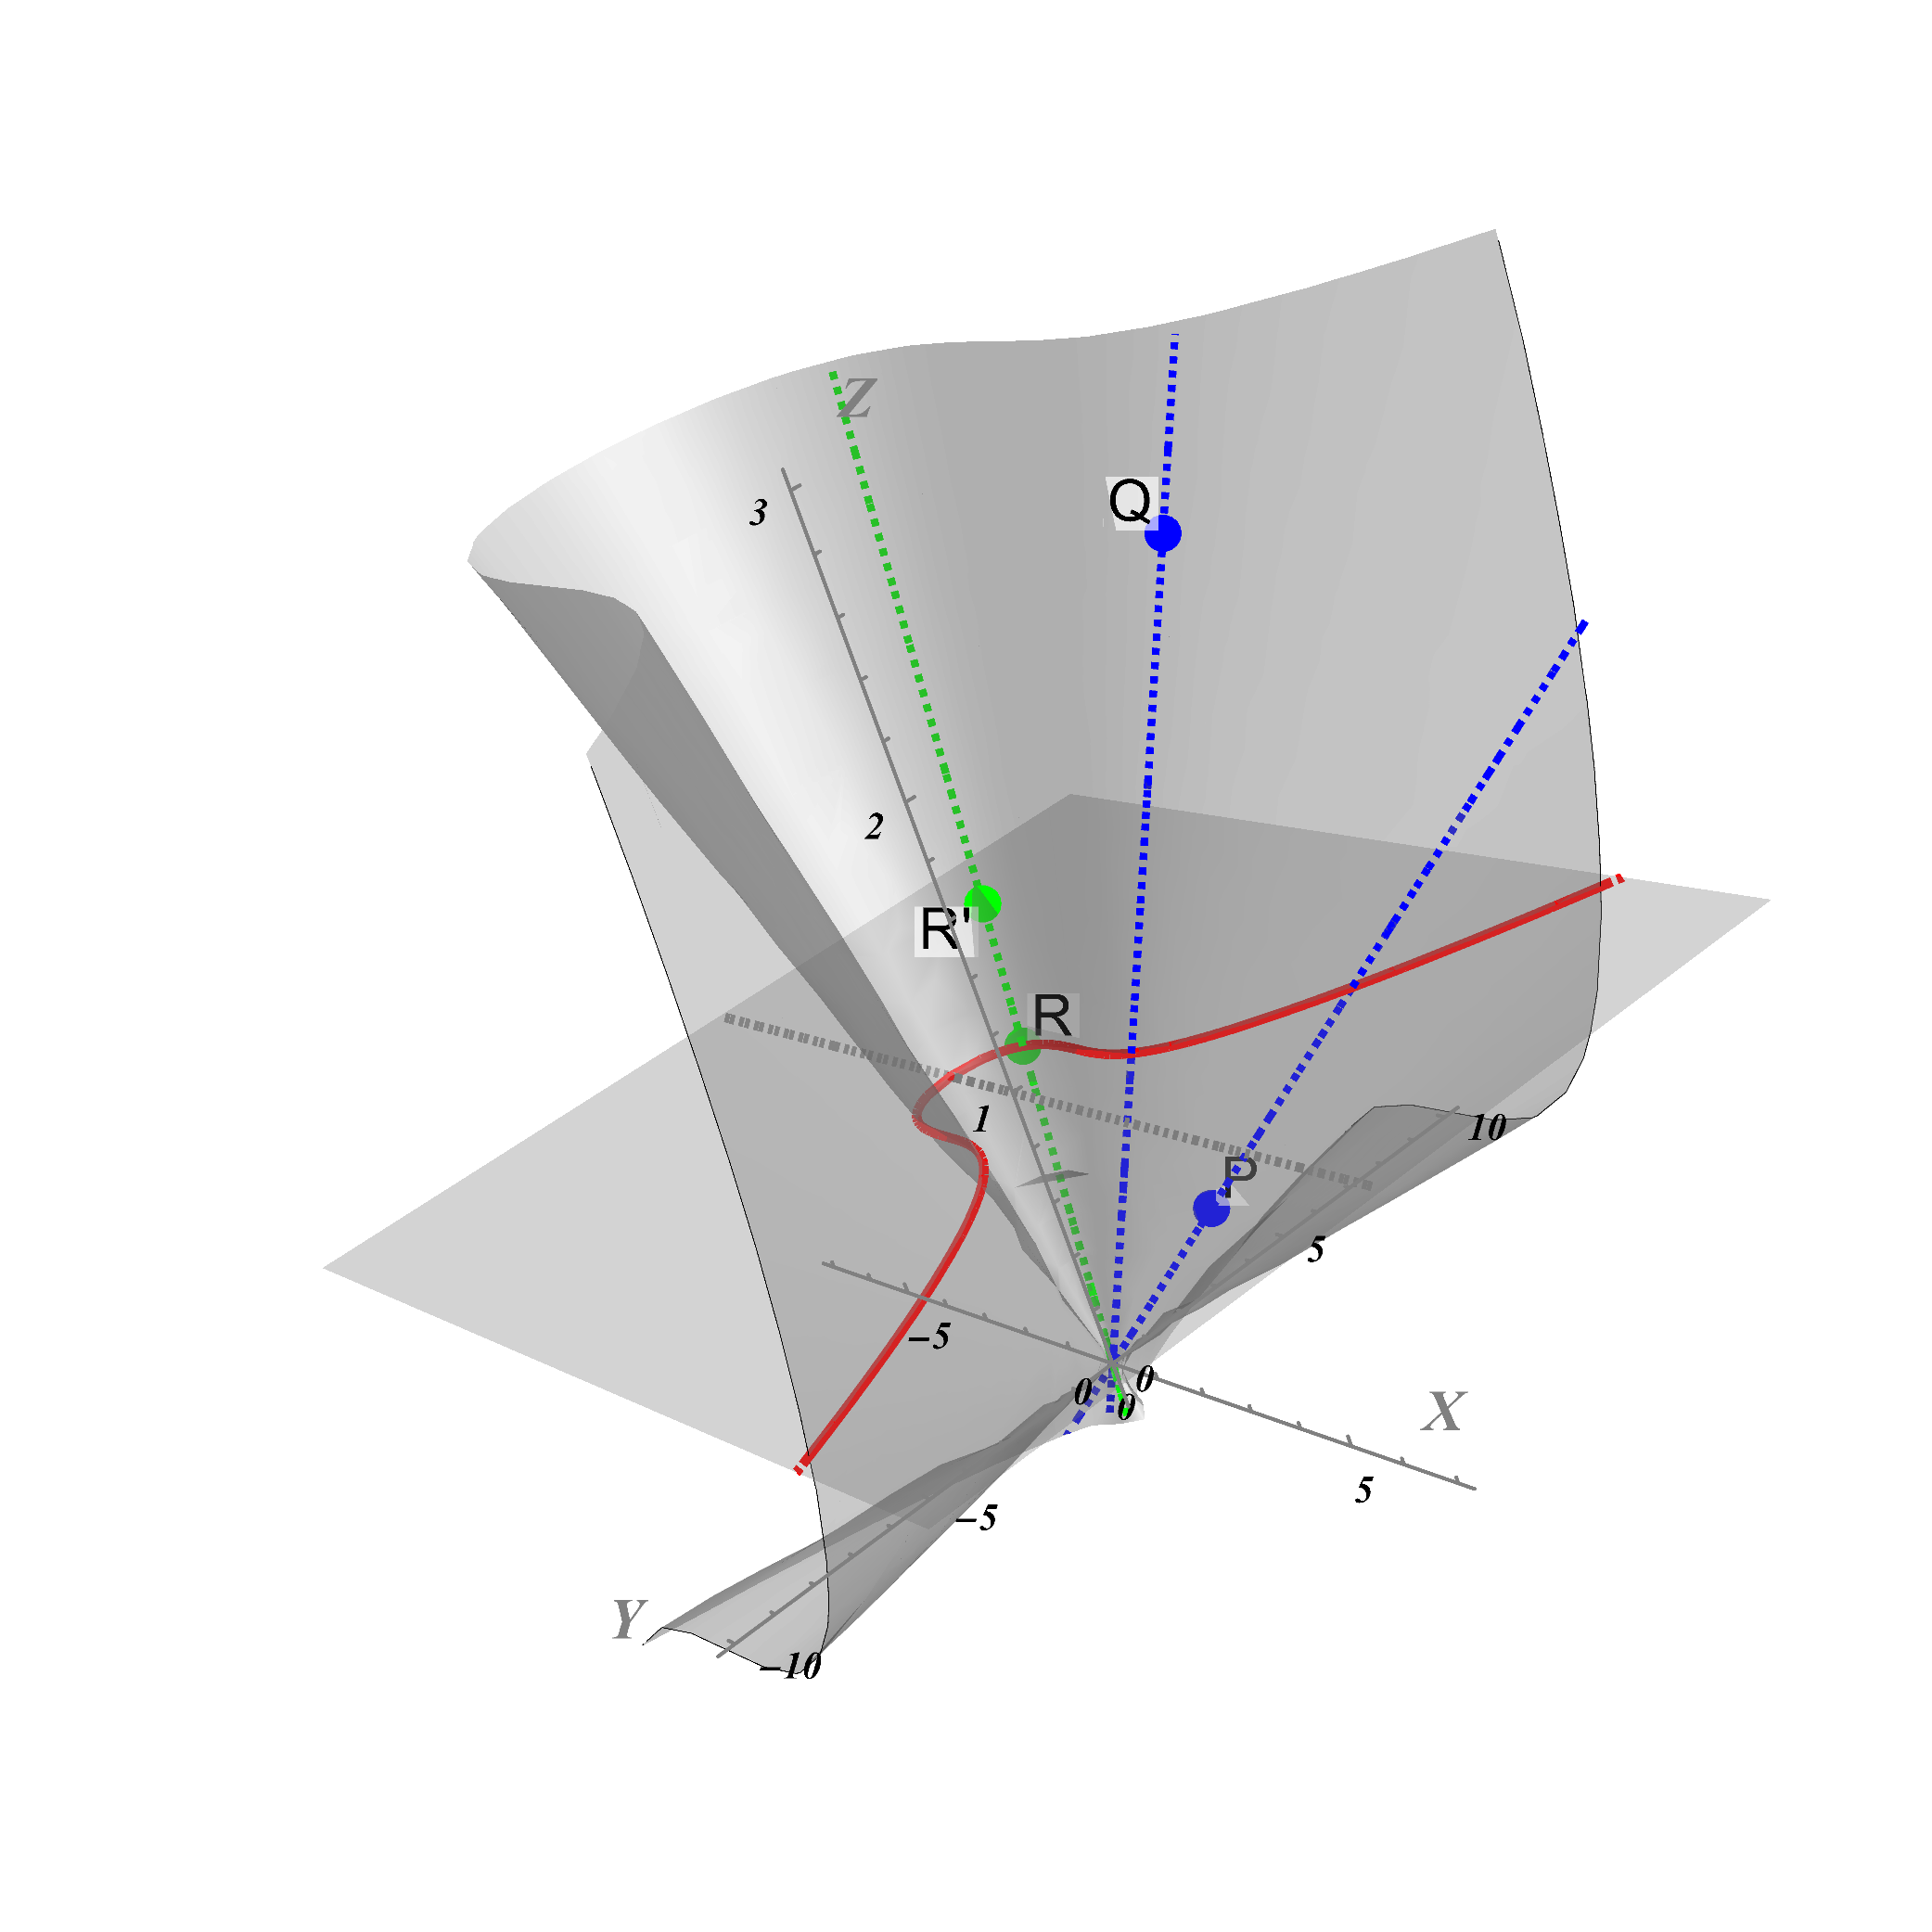
\includegraphics[width=0.75\textwidth]{images/lecture_4/ecadd.pdf}
        \end{figure}
    \end{frame}

    \begin{frame}{General Strategy}
        \begin{enumerate}
            \item Convert affine form $(X_P,Y_P)$ to the projective $(X_P:Y_P:1)$.
            \item Make many additions, doubling, multiplications etc. in projective form, getting $(X_R:Y_R:Z_R)$ at the end.
            \item Convert back to affine coordinates:
            \begin{equation*}
                (X_R:Y_R:Z_R) \mapsto (X_R/Z_R,Y_R/Z_R)
            \end{equation*}
        \end{enumerate}

        \begin{figure}
            \centering
            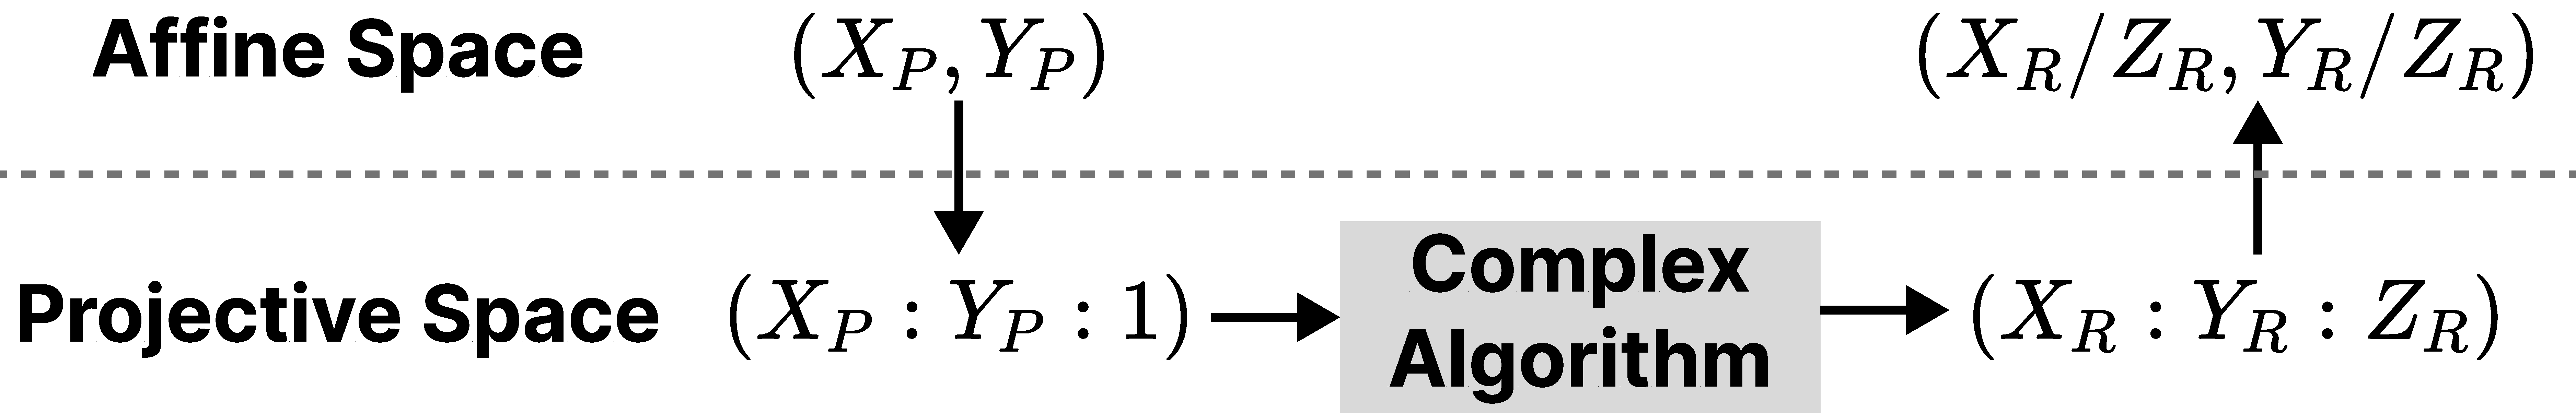
\includegraphics[width=\textwidth]{images/lecture_4/strategy.pdf}
            \caption{General strategy with EC operations.}
        \end{figure}
    \end{frame}

    \begin{frame}{General Projective Coordinates}
        \begin{gather*}
            (X:Y:Z) \sim (X':Y':Z') \;\; \text{iff} \\ \exists \lambda \in \overline{\mathbb{K}}: (X,Y,Z) = (\lambda^n X', \lambda^m Y', \lambda Z')
        \end{gather*}
        
         In this case, to come back to the affine form, we need to use the map $\phi: (X:Y:Z) \mapsto (X/Z^n, Y/Z^m)$. 
         \begin{example}
            The case $n=2,m=3$ is called the \textbf{Jacobian Projective Coordinates}. An Elliptic Curve equation might be then rewritten as: 
            \begin{equation*}
                Y^2 = X^3 + aXZ^4 + bZ^6
            \end{equation*}
        \end{example}
    \end{frame}

    \begin{frame}{Illustration of General Projective Coordinates}
        \begin{example}
            Consider the BN254 curve $y^2 = x^3 + 3$ over reals $\mathbb{R}$, again. Its \textit{Jacobian projective form} is given by $Y^2 = X^3 + 3Z^6$.
            \begin{center}
                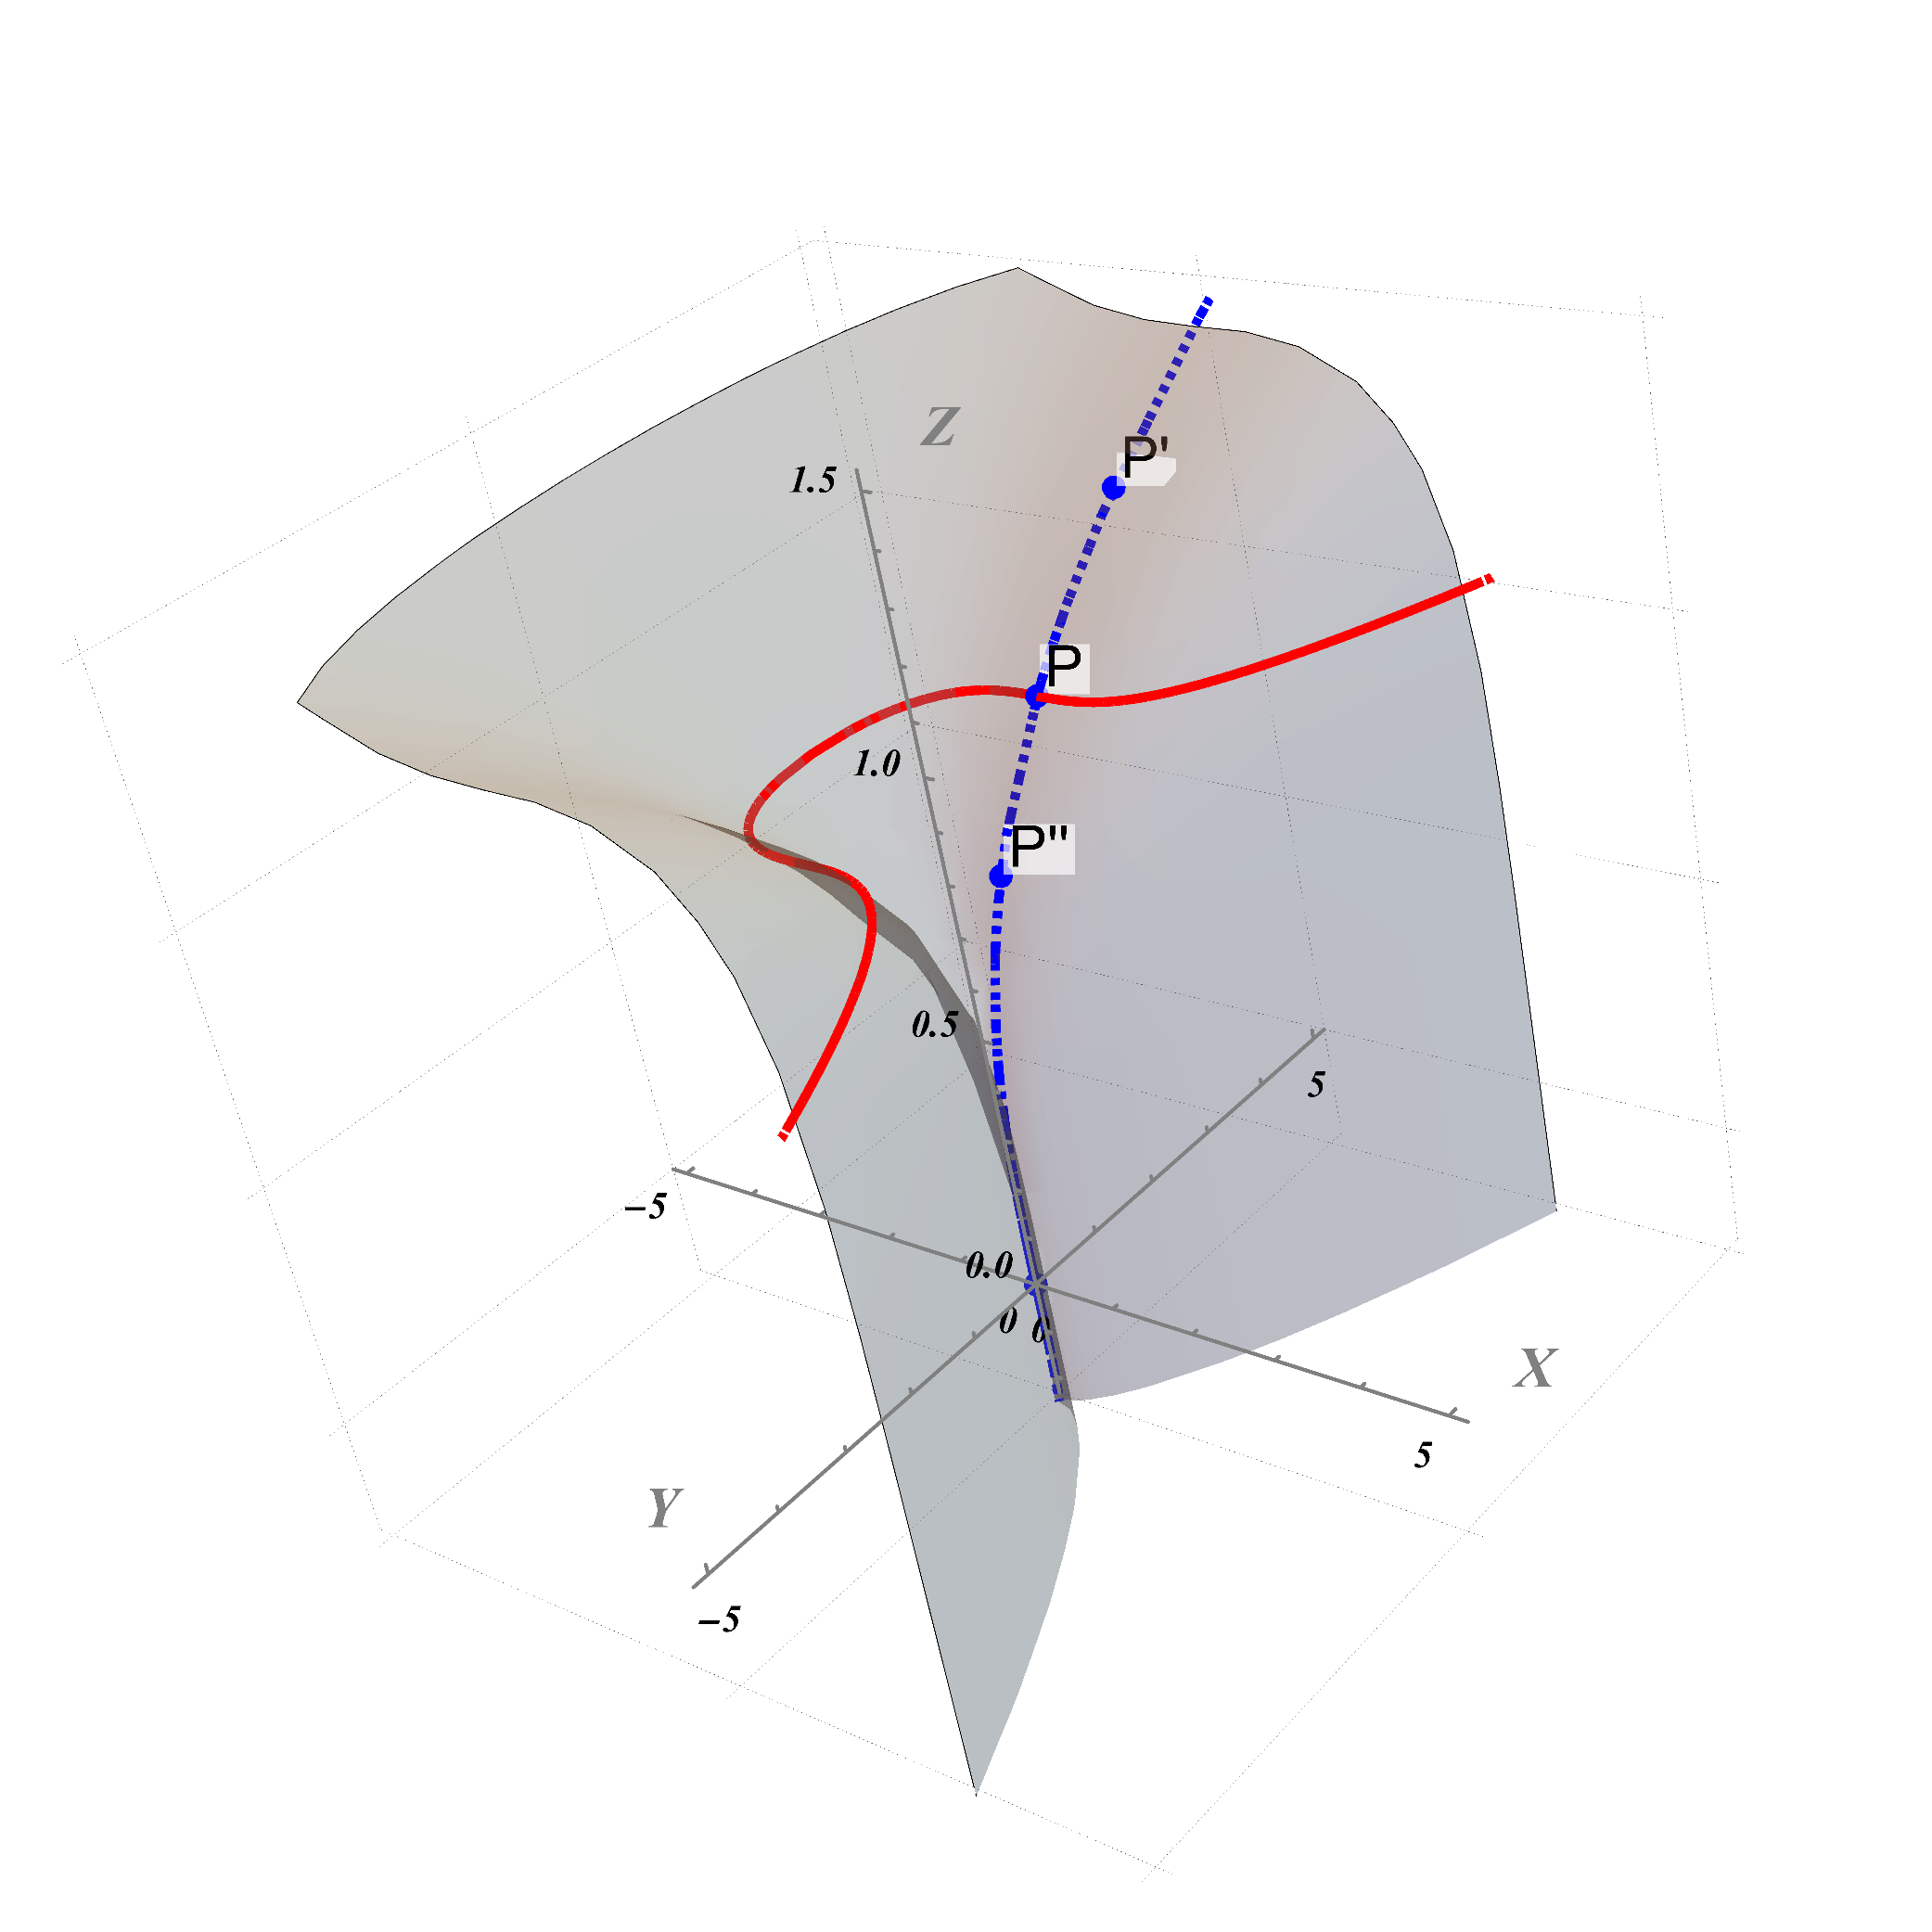
\includegraphics[trim={275 140 225 100}, width=0.3\linewidth, clip]{images/lecture_4/projective_ec_jacobian.pdf}
                
            \end{center}
        \end{example}
    \end{frame}

    \section{Elliptic Curve-based Pairing}
    \begin{frame}{Definition}
        \begin{definition}
            \textbf{Pairing} is a bilinear, non-degenerate, efficiently computable map $e: \textcolor{oc-red-7}{\mathbb{G}_1} \times \textcolor{oc-indigo-8}{\mathbb{G}_2} \to \textcolor{oc-green-8}{\mathbb{G}_T}$, where $\textcolor{oc-red-7}{\mathbb{G}_1},\textcolor{oc-indigo-8}{\mathbb{G}_2}$ are two groups (typically, elliptic curve groups) and $\textcolor{oc-green-8}{\mathbb{G}_T}$ is a target group (typically, a set of scalars). Let us decipher the definition:
            \begin{itemize}
                \item \textbf{Bilinearity} means essentially the following:
                \begin{equation*}
                    e([a]\textcolor{oc-red-7}{P},[b]\textcolor{oc-indigo-8}{Q}) = e([ab]\textcolor{oc-red-7}{P},\textcolor{oc-indigo-8}{Q}) = e(\textcolor{oc-red-7}{P},[ab]\textcolor{oc-indigo-8}{Q}) = e(\textcolor{oc-red-7}{P},\textcolor{oc-indigo-8}{Q})^{ab}.        
                \end{equation*}
                \item \textbf{Non-degeneracy} means that $e(G_1,G_2) \neq 1$ (where $G_1,G_2$ are generators of $\textcolor{oc-red-7}{\mathbb{G}_1},\textcolor{oc-indigo-8}{\mathbb{G}_2}$, respectively). This property basically says that the pairing is not trivial.
                \item \textbf{Efficient computability} means that the pairing can be computed in a reasonable time.
            \end{itemize}
        \end{definition}
    \end{frame}

    \begin{frame}{Primitive Example}
        \begin{example}
            Suppose $\mathbb{G}_1=\mathbb{G}_2=\mathbb{G}_T=\mathbb{Z}_r$ are scalars. Then, the following map $e: \mathbb{G}_1 \times \mathbb{G}_2 \to \mathbb{G}_T$ is a pairing:
            \begin{equation*}
                e(x,y)= 2^{xy}
            \end{equation*}
            \begin{itemize}
                \item \textbf{Bilinearity:}
                \begin{gather*}
                    e(ax,by) = 2^{abxy} = (2^{xy})^{ab} = e(x,y)^{ab} \\
                    e(ax,by)=2^{abxy}=2^{(x)(aby)}=e(x,aby)
                \end{gather*}
                \item \textbf{Non-degeneracy:} $e(1,1)=2 \neq 1$.
                \item \textbf{Efficient computability:} Obvious.
            \end{itemize}    
        \end{example}
    \end{frame}

    \begin{frame}{Elliptic Curve-based Pairing}
        \begin{example}
            \textbf{Pairing for BN254.} For BN254 (with equation $y^2=x^3+3$), the pairing function $e: \textcolor{oc-red-7}{\mathbb{G}_1} \times \textcolor{oc-indigo-8}{\mathbb{G}_2} \to \textcolor{oc-green-8}{\mathbb{G}_T}$ is defined over the following groups:
            \begin{itemize}
                \item $\textcolor{oc-red-7}{\mathbb{G}_1}$ --- points on the regular curve $E(\mathbb{F}_p)$.
                \item $\textcolor{oc-indigo-8}{\mathbb{G}_2}$ --- $r$-torsion points on the twisted curve $E'(\mathbb{F}_{p^2})$ over the field extension $\mathbb{F}_{p^2}$ (with equation $y^2 = x^3+\frac{3}{\xi}$ for $\xi=9+u \in \mathbb{F}_{p^2}$).
                \item $\textcolor{oc-green-8}{\mathbb{G}_T}$ --- $r$th roots of unity $\Omega_r \subset \mathbb{F}_{p^{12}}^{\times}$.
            \end{itemize}
        
             Some clarifications:
            \begin{itemize}
                \item \textbf{$r$-torsion subgroup}: $E(\mathbb{F}_{p^m})[r] = \{P \in E(\mathbb{F}_{p^m}): [r]P = \mathcal{O}\}$.
                \item \textbf{$r$th roots of unity}: $\Omega_r = \{z \in \mathbb{F}_{p^{12}}^{\times}: z^r=1\}$.
            \end{itemize}
        \end{example}

        \begin{alertblock}{Question}
            If $E(\mathbb{F}_p)$ is cyclic, $r=|E(\mathbb{F}_p)|$, what is $E(\mathbb{F}_p)[r]$?
        \end{alertblock}
    \end{frame}
    
    \begin{frame}{EC Pairing Illustration}
        \begin{figure}
            \centering
            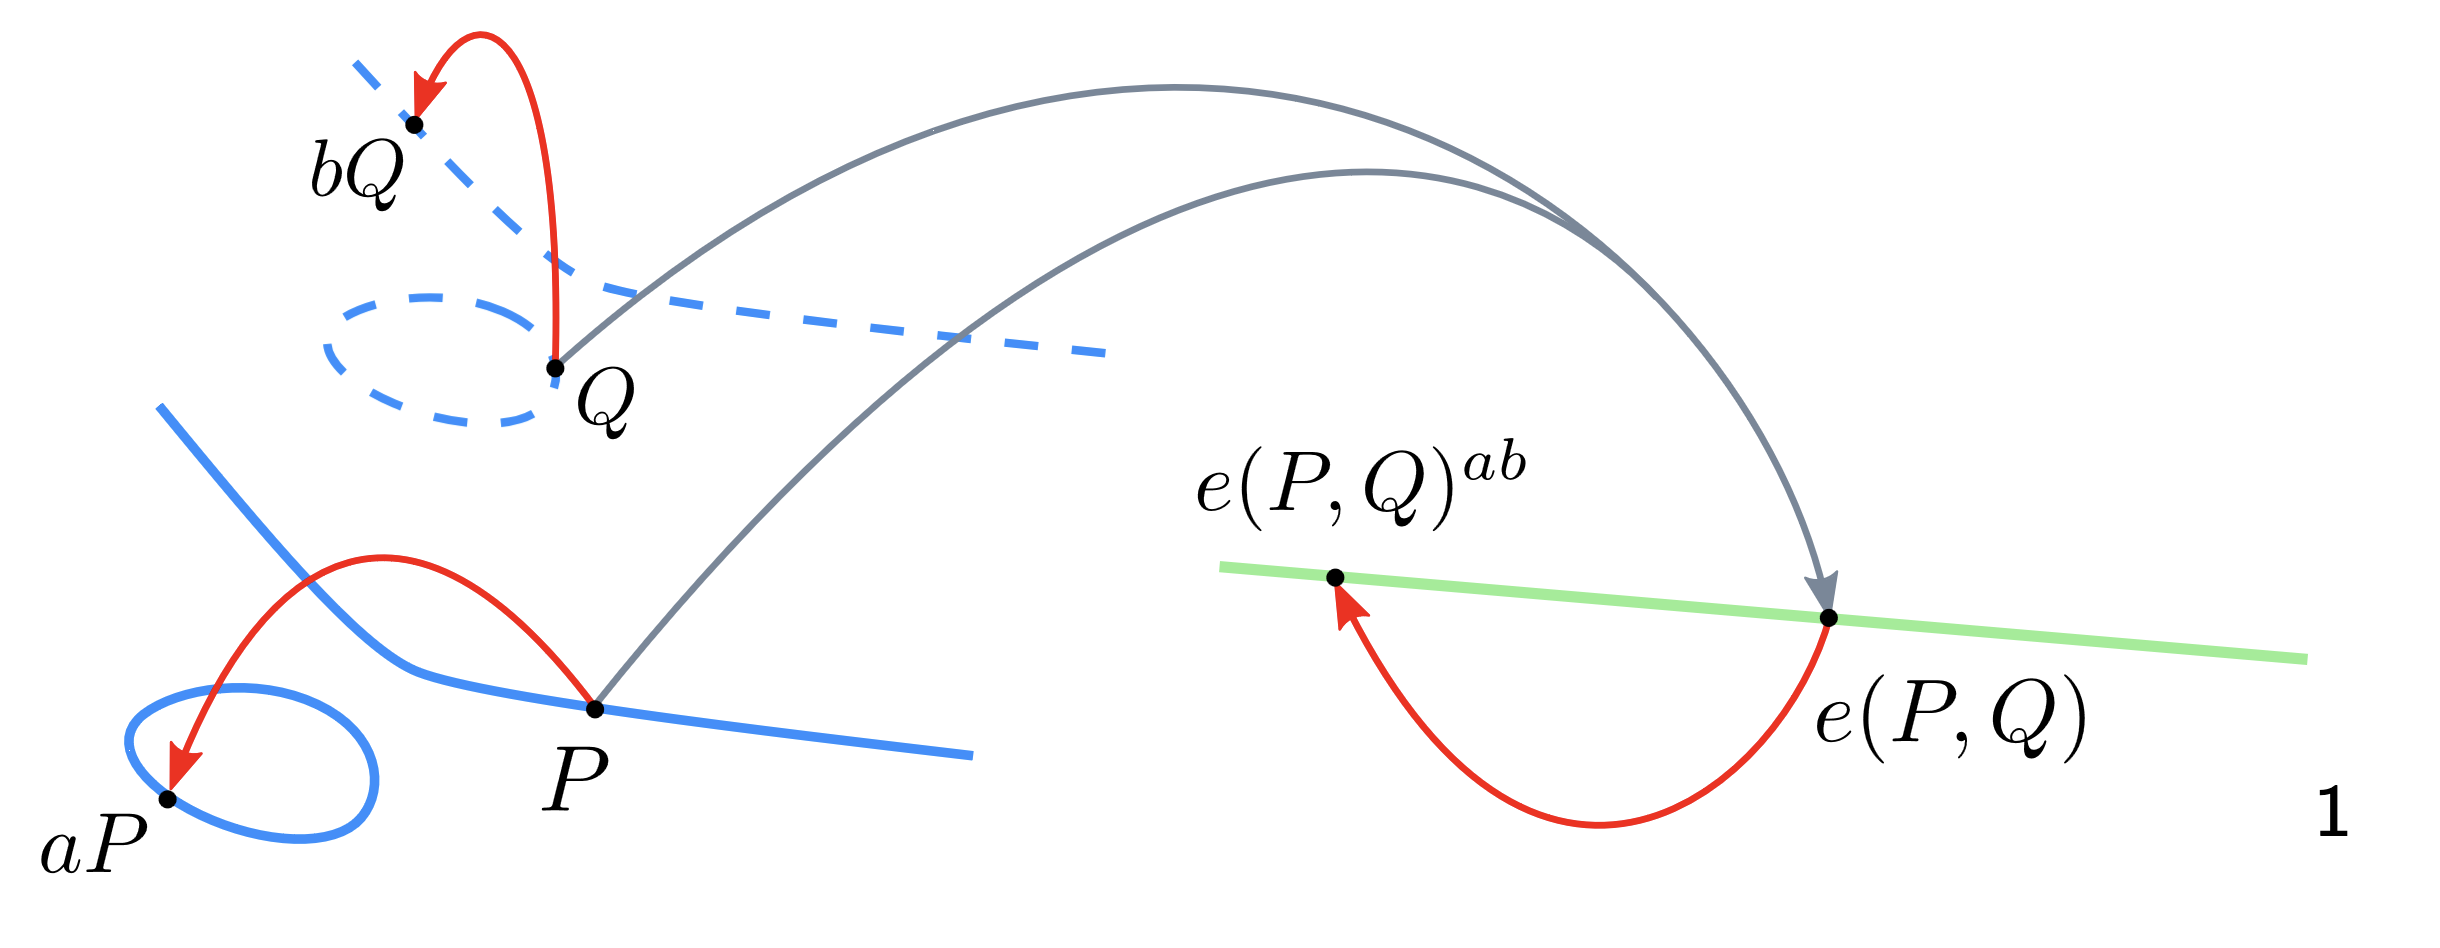
\includegraphics[width=\textwidth]{images/lecture_4/pairing.png}
            \caption{Pairing illustration. It does not matter what we do first: (a) compute $[a]P$ and $[b]Q$ and then compute $e([a]P,[b]Q)$ or (b) first calculate $e(P,Q)$ and then transform it to $e(P,Q)^{ab}$.}
        \end{figure}
    \end{frame}

    \begin{frame}{Pairing-friendliness}
        \begin{block}{Remark}
            One might have a reasonable question: where does this $12$ come from? The answer is following: the so-called \textbf{embedding degree} of BN254 curve is $k=12$.
        \end{block}
        
        \begin{definition}
            The following conditions are equivalent \textbf{definitions} of an embedding degree $k$ of an elliptic curve $E(\overline{\mathbb{F}}_p)$:
            \begin{itemize}
                \item $k$ is the smallest positive integer such that $r \mid (p^k-1)$.
                \item $k$ is the smallest positive integer such that $\mathbb{F}_{p^k}$ contains all of the $r$-th roots of unity in $\overline{\mathbb{F}}_p$, that is $\Omega_r \subset \mathbb{F}_{p^k}$.
                \item $k$ is the smallest positive integer such that $E(\overline{\mathbb{F}}_p)[r] \subset E(\mathbb{F}_{p^k})$
            \end{itemize}
             An elliptic curve is called \textbf{pairing-friendly} if it has a relatively small embedding degree $k$ (typically, $k \leq 16$).
        \end{definition}
    \end{frame}

    \begin{frame}{Application \#1: BLS Signature}
        Suppose we have pairing $e: \mathbb{G}_1 \times \mathbb{G}_2 \to \mathbb{G}_T$ (with generators $G_1,G_2$, respectively), and a hash function $\mathsf{H}$, mapping message space $\mathcal{M}$ to $\mathbb{G}_1$.
        
        \begin{block}{Definition}
            \textbf{BLS Signature} consists of the following algorithms:
            \begin{itemize}
                \item $\mathsf{Gen}(\cdot)$: Key generation. $\mathsf{sk} \xleftarrow[]{R} \mathbb{Z}_q, \mathsf{pk} \gets [\mathsf{sk}] G_2 \in \mathbb{G}_2$.
                \item $\mathsf{Sign}(\mathsf{sk},m)$. Signature is $\sigma \gets [\mathsf{sk}] \mathsf{H}(m) \in \mathbb{G}_1$.
                \item $\mathsf{Verify}(\mathsf{pk},m,\sigma)$. Check whether $e(\mathsf{H}(m), \mathsf{pk}) = e(\sigma, G_2)$. 
            \end{itemize}
        \end{block}
        
        Let us check the correctness:
        \begin{equation*}
            e(\sigma,G_2) = e(\textcolor{oc-indigo-8}{[\mathsf{sk}]}\mathsf{H}(m),G_2) = e(\mathsf{H}(m), \textcolor{oc-indigo-8}{[\mathsf{sk}]}G_2) = e(\mathsf{H}(m), \mathsf{pk})
        \end{equation*}
        
        \textbf{Remark:} $\mathbb{G}_1$ and $\mathbb{G}_2$ might be switched: public keys might live instead in $\mathbb{G}_1$ while signatures in $\mathbb{G}_2$.
    \end{frame}

    \begin{frame}{Application \#2: Quadratic Verifications}
        \begin{block}{Task}
            Alice wants to convince Bob that she knows such $\alpha,\beta$ such that $\alpha + \beta = 2$, but she does not want to reveal $\alpha,\beta$. How to do that?
        \end{block}

        \begin{example}
            \begin{enumerate}
                \item Alice computes $P \gets [\alpha]G, Q \gets [\beta]G$ --- points on the curve.
                \item  Alice sends $(P,Q)$ to Bob.
                \item  Bob verifies whether $P\oplus Q = [2]G$.
            \end{enumerate}
            
             Let us verify the \textbf{correctness:} 
            \begin{equation*}
                P\oplus Q = [\alpha]G \oplus [\beta]G = [\alpha+\beta]G = [2]G
            \end{equation*}
        \end{example}
    \end{frame}

    \begin{frame}{Application \#2: Quadratic Verifications}
        \begin{block}{Task}
            Alice wants to convince that she knows $\alpha,\beta$ such that $\alpha\beta=2$ without revealing $\alpha,\beta$.
        \end{block}

        \begin{example}
            \begin{enumerate}
                \item Alice computes $P \gets [\alpha]G_1 \in \mathbb{G}_1, Q \gets [\beta]G_2 \in \mathbb{G}_2$ --- points on two curves.
                \item  Alice sends $(P,Q) \in \mathbb{G}_1 \times \mathbb{G}_2$ to Bob.
                \item  Bob checks whether: $e(P,Q) = e(G_1,G_2)^{2}$.
            \end{enumerate}
            
             Again let us verify the \textbf{correctness:} 
            \begin{equation*}
                e(P,Q) = e([\alpha]G_1,[\beta]G_2) = e(G_1,G_2)^{\alpha\beta} = e(G_1,G_2)^{2}
            \end{equation*}
        \end{example}
    \end{frame}

    \begin{frame}{Application \#2: Quadratic Verifications}
        \begin{block}{Task}
            Alice wants to convince that she knows $x_1,x_2$ such that $x_1^2+x_1x_2=x_2$ without revealing $x_1,x_2$.
        \end{block}

        \begin{example}
            Alice calculates $P_1 \gets [x_1]G_1 \in \mathbb{G}_1$, $P_2 \gets [x_1]G_2 \in \mathbb{G}_2$, $Q \gets [x_2]G_2 \in \mathbb{G}_2$. Then, the condition can be verified by checking whether
            \begin{equation*}
                e(P_1,P_2\oplus Q)e(G_1,\ominus Q) = 1
            \end{equation*}
             Let us see the correctness of this equation:
            \begin{gather*}
                e(P_1,P_2\oplus Q)e(G_1,\ominus Q) = e([x_1]G_1,[x_1+x_2]G_2)e(G_1,[x_2]G_2)^{-1} \nonumber \\= e(G_1,G_2)^{x_1(x_1+x_2)}e(G_1,G_2)^{-x_2} = e(G_1,G_2)^{x_1^2+x_1x_2-x_2}
            \end{gather*}
        \end{example}
    \end{frame}
    
    \begin{frame}[plain, standout]
        \centering
        \LARGE
        \textbf{Thank you for your attention} \\
        
        \vspace{0.2cm} \Huge \ding{170} \large \\
        
        \vspace{1cm}
  
        \href{https://zkdl-camp.github.io/}{\raisebox{-.1em}{\hspace{.025em}\faIcon{globe}}\hspace{.325em}zkdl-camp.github.io} \\
  
        \href{https://github.com/ZKDL-Camp}{\raisebox{-.1em}{\hspace{.025em}\faIcon{github}}\hspace{.325em}github.com/ZKDL-Camp}
        
        \begin{center}
            
\includegraphics[width=0.15\textwidth]{images/logo.png}
        \end{center}
    \end{frame}
\end{document}